% arara: xelatex
% arara: bibtex
% arara: xelatex
% arara: xelatex

% Pattern Languages of Programs Conference 2023 October 22-25, 2023

% Original timeline:

% June 2         Shepherding begins
%% - We'll know if we have a shepherd
% June 30        Deadline focus group / workshop proposals
% August 7       Second draft due for review
% August 15      Notification of acceptance
% September 18   Conference versions due
% October 1      Conference registration ends
% October 22     Patterns Bootcamp
% October 23-25  PLoP Conference Days

% January 29, 2024 Proceeding version due

% Created 2021-11-16 Tue 16:22
% Intended LaTeX compiler: xelatex
\RequirePackage[prologue,table]{xcolor}
\documentclass[acmlarge,timestamp]{acmart}

\usepackage[many]{tcolorbox}
\usepackage{varwidth}
\usepackage{environ}
\usepackage{xparse}
\usepackage{microtype}

\newlength{\bubblewidth}
\AtBeginDocument{\setlength{\bubblewidth}{.75\textwidth}}
\definecolor{bubblegreen}{rgb}{0.67, 0.9, 0.93}
\definecolor{bubblegray}{RGB}{241,240,240}

\newcommand{\bubble}[4]{%
  \tcbox[
    colback=#1,
    colframe=#1,
    #2,
  ]{\color{#3}\begin{varwidth}{\bubblewidth}#4\end{varwidth}}%
}

\ExplSyntaxOn
\seq_new:N \l__ooker_bubbles_seq
\tl_new:N \l__ooker_bubbles_first_tl
\tl_new:N \l__ooker_bubbles_last_tl

\NewEnviron{rightbubbles}
 {
  \raggedleft\sffamily
  \seq_set_split:NnV \l__ooker_bubbles_seq { \par } \BODY
  \int_compare:nTF { \seq_count:N \l__ooker_bubbles_seq < 2 }
   {
    \bubble{bubblegreen}{rounded~corners}{black}{\BODY}
   }
   {
    \seq_pop_left:NN \l__ooker_bubbles_seq \l__ooker_bubbles_first_tl
    \seq_pop_right:NN \l__ooker_bubbles_seq \l__ooker_bubbles_last_tl
    \bubble{bubblegreen}{sharp~corners=southeast}{black}{\l__ooker_bubbles_first_tl}\par
    \seq_map_inline:Nn \l__ooker_bubbles_seq
     {
      \bubble{bubblegreen}{sharp~corners=east}{black}{##1}\par
     }
    \bubble{bubblegreen}{sharp~corners=northeast}{black}{\l__ooker_bubbles_last_tl}\par
   }
 }
\NewEnviron{leftbubbles}
 {
  \raggedright\sffamily
  \seq_set_split:NnV \l__ooker_bubbles_seq { \par } \BODY
  \int_compare:nTF { \seq_count:N \l__ooker_bubbles_seq < 2 }
   {
    \bubble{bubblegray}{rounded~corners}{black}{\BODY}
   }
   {
    \seq_pop_left:NN \l__ooker_bubbles_seq \l__ooker_bubbles_first_tl
    \seq_pop_right:NN \l__ooker_bubbles_seq \l__ooker_bubbles_last_tl
    \bubble{bubblegray}{sharp~corners=southwest}{black}{\l__ooker_bubbles_first_tl}\par
    \seq_map_inline:Nn \l__ooker_bubbles_seq
     {
      \bubble{bubblegray}{sharp~corners=west}{black}{##1}\par
     }
    \bubble{bubblegray}{sharp~corners=northwest}{black}{\l__ooker_bubbles_last_tl}\par
   }
 }
\ExplSyntaxOff

%%%

\newfontfamily{\chess}[Color=red]{chess_merida_unicode.ttf}
%\newfontfamily{\emoji}[Color=red]{DejaVu Sans}

\usepackage{xltxtra}
\usepackage{slantsc}
%\usepackage{xelatexemoji}
%\renewcommand{\xelatexemojipath}[1]{./svg/U#1.PDF}

\setcopyright{rightsretained}
\copyrightyear{2021}
\acmYear{2021}
\acmDOI{10.XXXX/XXXXXXX.XXXXXXX}

%% These commands are for a PROCEEDINGS abstract or paper.
\acmConference[PLoP'23]{PLoP'23: Pattern Languages of Programs 2023}{October 23--25, 2023}{HILLSIDE}
\acmBooktitle{PLoP'23, OCTOBER 5--7, HILLSIDE. Copyright 2023 is held by the author(s)}
\acmPrice{15.00}
\acmISBN{978-1-4503-XXXX-X/18/06}

%\usepackage[Latin,Greek,Emoticons]{ucharclasses}
\usepackage{graphicx}
\usepackage{grffile}
\usepackage{longtable}
\usepackage{wrapfig}
\usepackage{rotating}
\usepackage[normalem]{ulem}
%\usepackage{amsmath}
\usepackage{textcomp}
%\usepackage{amssymb}
\usepackage{capt-of}
\usepackage{hyperref}
\usepackage{fontspec}

%\newfontfamily\emoji[Path = /home/joe/PatternsOfPatternsII/]{Noto Color Emoji}

\usepackage{emoji}
\setemojifont{Noto Color Emoji}
%\usepackage{coloremoji}

\usepackage{mdframed}
\usepackage{afterpage}

\usepackage{booktabs}
%\usepackage[]{xcolor} %for use in color links
%\usepackage{colortbl}

\usepackage[pagewise]{lineno}
\renewcommand\thelinenumber{\color{red}\arabic{linenumber}}
%\usepackage{xunicode}
\usepackage{natbib}
\usepackage{float}
%\usepackage{xypic}
\usepackage{tikz}
\newcommand{\sensory}{(s)}
\newcommand{\cognitive}{(c)}
\newcommand{\motor}{(m)}
\newcommand*\circlednum[1]{\resizebox{1em}{!}{\tikz[baseline=(char.base)]{\node[shape=circle,draw,inner sep=2pt] (char) {#1};}}}
%\usepackage{amsmath, amssymb}
\def\t{\scriptstyle\triangle}
\def\T{\textstyle\blacktriangle}
\usepackage{placeins}
%\usepackage{starfont}
% \newfontfamily{\alch}{Alchemy}
%\newcommand{\Asclepius}{{\emoji\symbol{"2695}}}
%\newcommand{\Caduceus}{{\emoji\symbol{"2624}}}
\setmainfont{Libertinus Sans}
\usepackage{bold-extra}
\DeclareRobustCommand{\scitshape}{\fontshape{\scitdefault}\selectfont}
\newenvironment{echo}{}{}
\usepackage{enotez}
\renewcommand{\endnote}[1]{}
\newcommand{\ignorelink}[2][]{#2}
\newcommand{\markbf}[1]{\textsuperscript{\textbf{#1}}}
\setenotez{counter-format = alph, mark-cs = \markbf}
\DeclareInstance{enotez-list}{sverre}{paragraph}{heading={},notes-sep=\baselineskip,format=\normalsize\normalfont\raggedright\leftskip1.8em,number=\makebox[0pt][r]{#1.\ }\ignorespaces,}
\usepackage{epigraph}
\date{}
\title{Patterns of Patterns II: Discourse on Implementation}
\hypersetup{
 pdfauthor={Joseph Corneli et al.},
 pdftitle={Patterns of Patterns II},
 pdfkeywords={},
 pdfsubject={},
 pdfcreator={Emacs 30.0.50 (Org mode 9.6.1)},
 pdflang={English}}

\citestyle{acmauthoryear}
\let\cleardoublepage=\clearpage
\begin{document}

\title{Patterns of Patterns II}

\author{Joseph Corneli}
\authornote{Corresponding author, jcorneli@brookes.ac.uk.}
\email{jcorneli@brookes.ac.uk}
\orcid{1234-5678-9012}
\affiliation{%
  \institution{Oxford Brookes University}
  \streetaddress{Gipsy Lane}
  \city{Oxford}
  \country{UK}
  \postcode{OX3 0BP}
}

\author{Noorah Alhasan}
\author{Leo Vivier}
\author{Alex Murphy}
\author{Raymond S. Puzio}
%\authornotemark[1]
\email{rsp@hyperreal.enterprises}
\affiliation{%
  \institution{Hyperreal Enterprises Ltd}
  \streetaddress{81 St Clement’s St}
  \city{Oxford}
  \country{UK}
  \postcode{OX4 1AW}}

\author{Abby Tabor}
\affiliation{%
  \institution{University of the West of England}
  \streetaddress{Faculty of Health and Applied Sciences (HAS), Frenchay Campus, Coldharbour Lane}
  \city{Bristol}
  \state{England}
  \country{UK}
  \postcode{BS16 1QY}}
\email{abby.tabor@uwe.ac.uk}

%% \author{Vitor Bruno}
%% \affiliation{%
%%   \institution{Milestone English}
%%   \streetaddress{Rua Trieste 170, ap2}
%%   \city{Palhoca}
%%   \state{SC}
%%   \country{Brazil}
%%   \postcode{88132-227}}
%% \email{chief@milestoneenglishcourse.com}

%% % \author{Paola Ricaurte}
%% % \affiliation{%
%% %   \institution{Tecnologico de Monterrey}
%% %   \streetaddress{Calle del Puente 222 Col. Ejidos de Huipulco, Tlalpan}
%% %   \city{Mexico City}
%% %   \country{Mexico}
%% % }
%% % \email{pricaurt@tec.mx}

\author{Sridevi Ayloo}
\affiliation{%
  \institution{New York City College of Technology}
  \streetaddress{300 Jay St}
  \city{Brooklyn}
  \postcode{11201}
  \country{USA}
}
\email{pricaurt@tec.mx}

\author{Charlotte Pierce}
\affiliation{%
  \institution{Pierce Press}
  \streetaddress{PO Box 206}
  \city{Arlington MA}
  \country{USA}
  \postcode{02476}
}
\email{charlotte.pierce@gmail.com}

\author{Charles J. Danoff}
\affiliation{%
  \institution{Mr Danoff’s Teaching Laboratory}
 \streetaddress{PO Box 802738}
 \city{Chicago}
 \state{IL}
  \country{USA}
  \postcode{60680}}
\email{contact@mr.danoff.org}

\author{Mary Tedeschi}
\author{Manvinder Singh}
\author{Kajol Khetan}
\affiliation{%
  \institution{Baruch College}
 \streetaddress{PO Box 802738}
 \city{New York}
 \state{NY}
  \country{USA}
  \postcode{60680}}
\email{mtedeschi@pace.edu}


%%
%% By default, the full list of authors will be used in the page
%% headers. Often, this list is too long, and will overlap
%% other information printed in the page headers. This command allows
%% the author to define a more concise list
%% of authors' names for this purpose.
\renewcommand{\shortauthors}{Corneli et al.}


% (1) Review the intention: what do we expect to learn or make together?

% - Joe: Wanted to walk through the PoP paper with Rebecca, in order to help solidify my own grasp of the concepts and get her feedback.
% - Rebecca: This topic sounded interesting when you mentioned it and I wanted to learn about Pop

% (2) Establish what is happening: what and how are we learning?

% - Indeed we did speed through the paper, Rebecca pointed out a few places where there was friction with the wording or concepts, like ``PEER-TO-PEER'' and also suggested Operational Research and Strategy as an appropriate topic; mentioned “improvisatory” style
% - Interruptions were welcomed!
% - Rebecca: was hesitant to interrupt the narrative
% - This is a bit different from usual IEAI style...

% (3) What are some different perspectives on what’s happening?

% - Joe: appreciate the time Rebecca has put into this a lot, and I also think this was a good way to present the paper
% - Rebecca: I think you assume knowledge in the presentation, and I think you need to assume the listener (if they aren’t in the area) that they don’t know anything.  It wouldn’t be patronising to explain the basic concepts.

% (4) What did we learn or change?

% - Talking to Karl, he would reconise one of the areas (probably) but not necessarily the other two.  Everyone is going to be new to some of these concepts.
% - This was great as a ``final edit'' — we will also be able to edit this paper until December
% - RR: is it your aim to automate?

% (5) What else should we change going forward?

% - Joe: if it would be helpful to RR, I’d certainly be happy to meet again about these ideas
% - Would this (patterns of patterns) to actually be useful for ethical AI?
% - E.g., rethink in the context of moral machines

%%
%% The abstract is a short summary of the work to be presented in the
%% article.
% distributed peer-to-peer networks
\begin{abstract}
We review how our earlier theorization of pattern methods fares in the
wild.  The “wild” here included a graduate school classroom in New
York, a workshop at a transdisciplinary conference in Arizona, a
nascent citizen science project in Bristol, and a professional
development day for a university in Oxford.  We encountered unexpected
challenges such as working with students in a HyFlex classroom,
getting conference attendees to feel comfortable evaluating the
conference they were presently attending, and adapting our plans on
the fly when leading workshops with surprising attendee responses.  We
describe and refine pattern specifications that will help other
practitioners of patterns in their own forays into the wild.
\end{abstract}

%%
%% The code below is generated by the tool at http://dl.acm.org/ccs.cfm.
%% Please copy and paste the code instead of the example below.
%%
\begin{CCSXML}
<ccs2012>
<concept>
<concept_id>10003456</concept_id>
<concept_desc>Social and professional topics</concept_desc>
<concept_significance>500</concept_significance>
</concept>
<concept>
<concept_id>10011007.10011074.10011075</concept_id>
<concept_desc>Software and its engineering~Designing software</concept_desc>
<concept_significance>300</concept_significance>
</concept>
<concept>
<concept_id>10011007.10011074.10011134.10003559</concept_id>
<concept_desc>Software and its engineering~Open source model</concept_desc>
<concept_significance>300</concept_significance>
</concept>
<concept>
<concept_id>10010405.10010481</concept_id>
<concept_desc>Applied computing~Operations research</concept_desc>
<concept_significance>300</concept_significance>
</concept>
<concept>
<concept_id>10010147.10010341</concept_id>
<concept_desc>Computing methodologies~Modeling and simulation</concept_desc>
<concept_significance>100</concept_significance>
</concept>
</ccs2012>
\end{CCSXML}

\ccsdesc[500]{Social and professional topics}
\ccsdesc[300]{Software and its engineering~Designing software}
\ccsdesc[300]{Software and its engineering~Open source model}
\ccsdesc[300]{Applied computing~Operations research}
\ccsdesc[100]{Computing methodologies~Modeling and simulation}


%%
%% Keywords. The author(s) should pick words that accurately describe
%% the work being presented. Separate the keywords with commas.
\keywords{Design Patterns, Pattern Languages, Action Reviews, Futures
Studies, Causal Layered Analysis, Emacs, Free Software, Peeragogy,
Climate Change, Innovation, Anticipation}

%\authorsaddresses{This command processes the author and affiliation and title This command processes the author and affiliation and title This command processes the author and affiliation and title This command processes the author and affiliation and title}

%%
%% This command processes the author and affiliation and title
%% information and builds the first part of the formatted document.
\maketitle


%\clearpage

\section{Introduction}
\label{sec:org195e8e3}
\label{Introduction}

%% ACTUAL START OF THE PAPER
%% {\color{red}
%% The previous installation in this series presented a high-level
%% methodological synthesis that aimed to get at the heart of what design
%% patterns are \cite{patterns-of-patterns-i}.  Here, we want to talk
%% about how we have implemented the methods described previously, and
%% give some reflections on where things are going next.  We will begin with a
%% recapitulation of the main points made in the earlier paper.  In
%% short, “Patterns of Patterns” encapsulated everything we had to say
%% about design patterns with \emph{one} overall pattern which operated
%% at a very high level.  Here, we elaborate many practical patterns
%% which expand on the same theme.  This fully-fledged collection of
%% patterns of patterns can help you organise your work with Design
%% Pattern Language methods.}

Our paper “Patterns of Patterns” presented a high-level methodological
synthesis of three techniques from design, futures studies, and
learning management in the form of a design pattern called PLACARD
\cite{patterns-of-patterns-i}.  Since then, we have had opportunities
to deploy and further develop these methods in various contexts.  We
will describe some of these applications in the four case studies
below.  We have distilled this experience into a collection of
practical patterns which augment the earlier high-level PLACARD
pattern.  This fully-fledged collection of patterns of patterns can
help you organize your work with Design Pattern Language methods.

% \textbf{Note: We can build out the structure based on this thesis, to follow through in later paragraphs.  These things are initially very different!  Maybe add a ref to the psych people about how difficult it is to combine them.  Let's talk some about the difficulties whether or not we have successfully negotiated them.}

% Towards realizing the promise of design patterns, we aim for an excavation and reworking of the theory.

\section{Background}
\subsection{Recap of “Patterns of Patterns”}
\label{sec:org7c32ecc}

We introduced a synthesis of methods that operationalize the
“sensory”, “cognitive” and “motor” systems from psychology in the context of social intelligence.  The particular methods we outlined were certainly not the only way to implement these system features.  What drew our attention is that each of the methods we selected comes with a framework or template; each of the methods is, essentially, a design pattern.

\begin{itemize}
\item Project Action Review (PAR): \emph{a set of five review questions to explore at a project checkpoint}.
\item Causal Layered Analysis (CLA): \emph{a set of four “layers” that can
be used to unpack a problem area of interest.}
\item Design Pattern Languages (DPL): \emph{each constituent pattern follows a “Context/Problem/Solution” template.}
\end{itemize}

We made the further assertion that these sensory, cognitive, and motor
methods can be hooked together, theorizing design patterns as little
pieces of moveable social intelligence.  We called the specific method
that combines PAR, CLA, and DPL the “PLACARD” pattern.

We applied these methods to analyze the design Pattern Language
literature and practices, and also developed a case study examining
the way the Emacs Research Group used related methods.  We built on
these analyzes to outline potential futures for the development of
pattern methods.
%% \begin{itemize}
%% \item PLACARD becomes transferable and computational.
%% \item Pattern language authoring communities move to free/libre/open
%%   source licensing
%% \item Patterns empower individuals and communities
%% \item Patterns facilitate economic empowerment
%% \end{itemize}
%% All of these potential futures have early indicators attached to them,
%% in the sense of William Gibson: “the future is already here, it’s just
%% not very evenly distributed”.  But, now with reference to Alan Turing, much
%% remains to be done.

\subsection{Related work}
Our work on this paper, and the prequel, progressed alongside the
Peeragogy project.\footnote{\url{https://peeragogy.org/}} Aspects of
peeragogy were previously presented as design patterns
\cite{corneli2015a}.  This paper focuses on a series of workshops that
made our style of working accessible for “{\scitshape Newcomer}\hspace{.05em}s\hspace{.05em}” to peeragogy.  In these workshops, and in the workshop series as
a whole, we co-created a context to study collaborative processes in
microcosm.

The overall aim of this line of work to study and support social
intelligence \cite{benkler2015peer}, with a particular emphasis on
learning aspects.  Design patterns are a useful medium for this work.
\citet{iba2016pattern} provide a large collection of patterns for
creating patterns; and their threefold decomposition of the pattern
language creation process, into mining (\emph{a sensory activity}),
writing (\emph{a cognitive activity}), and symbolizing (\emph{a motor
activity}), bears an analogy with PLACARD.  However, our aim is not to
retrace Iba and Isaku’s {\scitshape Pattern Language Creation} pattern
— though we do cross-reference their work at key junctures here.
Rather, we descibe our own process of working with patterns with the
aim of further developing our reconstruction of pattern theory.

Earlier authors, such as \citet{moran1971a} and \citet{OXMAN1994141},
looked at the specifically-computational implementation of design
pattern ideas.  Computational considerations remain mostly in the
background for us, as we focus on features of implementation at the
social interaction and paper prototype level.  We return to questions
related to supportive computational implementation in the closing
sections of this paper.

We will draw heuristic connections between design patterns and the
active inference framework, a theory originating in theoretical
neuroscience which “can be applied to explain the influential flows and
dynamics of any open system at any scale” \cite{Hiplito2022}.
Hip\'olito and van Es point out that patterns (when understood in a
suitably general sense) are pre-linguistic, and are discovered and
learned through bodily experience.  The articulation of patterns in
language supports a process of \emph{niche construction}.
%% Can we relate Alexander’s “Maximum Entropy” analysis with the stats methods used here?
%% Add City is not a tree quote.
%% In this regard, we work in a way that is rather closer to the
%% sensibilities of Christopher \citet{alexander1965a} —
%% \begin{quote}
%% It is more and more widely recognized today that there is some
%% essential ingredient missing from artificial cities. When compared
%% with ancient cities that have acquired the patina of life, our modern
%% attempts to create cities artificially are, from a human point of
%% view, entirely unsuccessful.
%% \end{quote}
%%—than those of Ren\'e
%% \citet{descartes1850discourse}, who wrote:
%% \begin{quote}
%% \ldots it is observable that the buildings which a single architect
%% has planned and executed, are generally more elegant and commodious
%% than those which several have attempted to improve, by making old
%% walls serve for purposes for which they were not originally built.
%% \end{quote}

Towards this end, we embrace the often messy process of prototyping
our way forward.  “Making old walls serve for purposes for which they
were not originally built” \cite{descartes1850discourse} is a suitable
metaphor for this process.  Whilst patterns have been thought of as a
“living language” \cite[p.~xvii]{alexander1977a} from the start, a
well-articulated evolutionary perspective on pattern language
development may be transformative at the practice level.  (In
particular, \citet[p.~xxiii]{lowy2019righting} notes that “no other
industry [apart from software development!] opts for a clean slate on
a regular basis simply because doing so does not make economic
sense.”)

\section{Methodology}
\label{sec:org134acbb}
\label{methods}

We ran three separate workshops that were inspired by the original set
of PLACARD methods, and we will describe how the methods evolved
further in those settings.  We also used “Patterns of Patterns” as a
focal reading over three sequential offerings of of a postgraduate
course, CIS 9590 “Information Systems Development Project” at Baruch
College, part of the City University of New York.  We use experience
reports, and Causal Layered Analysis \cite{inayatullah1998b}, to
develop a deep dive into that specific application.  We also used of
CLA as a tool in the other workshops, via a new visual template which
bears some similarity to the “wholeness egg” of
\citet{wholeness-egg-II}.

In developing the workshops, our central methodological technique was
to use design patterns—as design inputs, as in-workshop manipulatives,
and as analytic outputs—in each of the workshops.  A representative
selection of these are included in this paper.  Each of the patterns
is given a marker, (s), (c), or (m), to indicate whether it plays a
primarily sensory, cognitive, or motor role.  We also include the
itinerary for each of the workshops to help bring the reader into the
scene.

We endeavor to show our process of pattern-development within the
paper.  As such, the paper includes a combination of patterns that
follow a formal template, and proto-patterns, without substructure.
The latter are distinguished by a “\emoji{gem}” marker, which evokes the
concept of \emph{pattern mining}.  In our view, additional formality
does not always help with communication.  We endeavor to show how and
when it is helpful.  In Section \ref{cis-case-study}, we give some
examples which show how our {\sc Pattern Language Components} can add
structure to proto-patterns.  Appendix \ref{synthesis-of-form} gives
some further justification for including work at different levels of
formality, with reference to \citet{alexander1964notes}.  Some of the
(proto-)patterns that we present here were created by workshop
participants, rather than by the paper’s coauthors, and these are
distinguished by a “\emoji{pick}” marker.

For the patterns which are spelled out formally in the paper, we use
this simple variation on the classical “Context Problem Solution”
pattern template:
\smallskip

\begin{tabular}{lll}
\phantom{hellohellohello}& \textbf{Context} \ldots & {[}Summary of the working context{]}\\
\phantom{hellohellohello}&\textbf{If} \ldots\ \emph{BUT} \ldots & {[}A conflict, problem, or gap arising in this context{]}  \\
\phantom{hellohellohello}&\textbf{Then} \ldots & {[}Actions to take to resolve the conflict{]}
\end{tabular}
\smallskip

We use an intuitive alternative template structure to describe a
sub-language of roles in Section \ref{second-case-study}.  In the
paper’s subsections which focus on presenting patterns, additional
narrative appears in an italic font.

We present the patterns that we developed and used in chronological
order, insofar as this was possible in a retrospective reflection.  In
our iterative way of working, the workshop method itself becomes a
kind of (complex) pattern, which we ran with variations.  At each
stage, input patterns play the role of lightweight hypotheses,
structuring the experience and potentially being validated or
invalidated by the interactions.  As observed by
\citet{iba2016pattern} the clear articulation of pattern-writing
patterns helps to identify when patterns are used: but \emph{not every
pattern is used every time}.  In our context, the survival of a given
pattern to the next workshop (or not) gives a sense of the
evolutionary character of the overall method.  The methodological
changes typically had a strategic rationale, and we aim to describe
this in our commentary.  We carefully reviewed the lessons learned
after each workshop, either by using the Project Action Review
template, or through less formal but nevertheless detailed post
mortems.  Writing this paper is linked with that aspect of the method,
since it provides the opportunity for review at a deeper rhythm.

If workshop development were our only aim, we would not have needed to
write this paper at all. \citet{miller-workshops} outlines a
general-purpose workshop design strategy.  Other methods which we have
encountered as workshop attendees include an adaptation of
\emph{sociocracy} \cite{sociocracy-manual}, a strategy for
collaboration that is distributed over nested ‘circles’, each of which
makes decisions by consent (rather than consensus); and \emph{theory
of change} \cite{Coryn2010}, a method for articulating criteria for a
project’s success.  General inspirations such as these are not
commented on specifically in the text, though we are confident that
they could be “patternized”.

\clearpage

\section{Case Study 1: “Going Meta” workshop at Anticipation 2022}\label{anticipation-case-study}

This workshop functioned as a more developed pilot of methods that we
shared at PLoP 2021 as “Flaws of the Cool
City”\footnote{\url{https://www.hillside.net/plop/2021/index.php?nav=program\#focusgroups}}
and at the Oxford Brookes Creative Industries Festival as “Dragon
versus monkey: A kaijū introduction to
peeragogy”\footnote{\url{https://www.brookes.ac.uk/research/networks/creative-industries-research-and-innovation/festival-2021}}
(and previously in more nascent forms).  Our aims were both to
introduce the methods to attendees, and to ‘workshop’ the methods.
Our pitch was that we would help attendees establish a position of
maximum leverage, exercising our “Critical Anticipatory Capacities”
using “Creativity, Innovation and New Media” (two of the conference’s
themes) to explore the future of anticipation.

\subsection{Input patterns} \label{case1-inputs}

\emph{The workshop activities were presented to workshop attendees in
the form of “pattern cards”.  A selection of these appear in Figure
\ref{cards}; several are detailed below, along with some more-abstract
patterns which were written down after the fact, but which characterize the
process that was used on the day.  The full collection of cards shared
with participants is available
online.\footnote{\url{https://hyperreal.enterprises/open-future/}}}
\emph{New cards were handed out for each phase of the workshop (for
the itinerary, see Section \ref{first-workshop-itinerary}), and were
color-coded accordingly.}

\begin{figure}
  \includegraphics[width=.9\textwidth,page=3,]{4-patternsa.pdf}
\caption{A selection of the pattern cards we handed out to participants of the “Going Meta” workshop\label{cards}}
\end{figure}

\subsection*{DÉRIVE COMIX{\hfill (s)}}

\textbf{Context} you want to develop some future scenarios to explore with a group.\newline
\textbf{If} the group has been identified BUT the members don’t know each other well yet, and accordingly each has their own separate experience, and the group has no concrete shared meanings;\newline
\textbf{Then} Gather data.  For example: go for a walk \cite{debord},  or just look out the window wherever you are.  (Alternatively, close your eyes and conduct a mental exploration of your selected theme: what do you see in “your mind’s eye?”) Document what you see.  Follow up by preparing your materials to share in a succinct fashion, e.g., as photos, a screenshot, slides, sketches, a zine, a map, or some PostIt\textsuperscript{\textregistered} notes.


\smallskip
\noindent \emph{By itself, looking at the immediate surroundings only
gives an imperfect picture of how to develop a future scenario.
Direct observations might include little to no evidence of, say,
top-level government policy which likely is a major factor in the
future.  Two further patterns work together to access more levels of
meaning:}

\subsection*{MEANING MAP {\hfill\cognitive}}

\textbf{Context} We have collected images describing people’s worlds
(see {\sc Dérive Comics}).\newline \textbf{If} you want to distill
well-integrated shared understandings for the group BUT, so far,
everyone has been keeping their experience, knowledge, and
perspectives to themselves;\newline \textbf{Then} talk together about
the problems and opportunities that everyone sees in the data that has
been shared, and document any connections you find.  Maybe some of the
themes will cluster together.  Maybe everyone will have wildly
different perspectives: that’s OK.  You can use these different
viewpoints to bring everyone on the same page: just document them as
part of the map.


\subsection*{REINFUSE EXPERTISE {\hfill \motor}}

\textbf{Context} a group wants to build a {\sc Meaning Map}.\newline
\textbf{If} everyone has experience as human being (and resident,
citizen, etc.) BUT they also have some experience as an expert which
is harder to share with non-experts;\newline \textbf{Then} begin by
removing expertise to get everyone on the same page, and subsequently
reinfuse expertise, to enable richer and more complex thinking.


\smallskip
\noindent \emph{The core process of informal sharing, map-making and
sharing knowledge works well in small groups.  A further level of
meaning can be accessed by sharing the key findings from small
groups.}

\subsection*{SHARE BACK {\hfill\sensory}}

\textbf{Context} Sub-groups have shared their experiences and each has
developed a {\sc Meaning Map} \newline \textbf{If} we want to
establish a meaning map for the whole group BUT unstructured
interaction within the whole room is infeasible;\newline \textbf{Then}
individual groups should present key findings to the room; or,
alternatively, if the conversations are not yet at a natural stopping
point ask the groups to pause their conversations and listen in briefly
to the one of groups (in turn), who will continue their small-group
conversation.


\smallskip
\noindent \emph{This nested process of sharing is intended to surface
the core themes that the group finds important.  In CLA terms, the
contents of the {\sc Share Back} are key inputs for the Myth layer.  A
facilitated whole-group discussion of how these core themes fit
together can yield a {\sc Meaning Map} which expresses the group’s
shared Myth.  At this point in the process, both the “zoomed out”
whole-group map, and the “zoomed in” small-group maps are likely to
contain ‘optative’ statements describing “the environment as we would
like it to be” \cite{zave1997four}, potentially also including
statements about what we wish not to have happen!  These are the seeds
of ‘scenarios’, though the details of these scenarios will only become
apparent as they are explored.  That happens in subsequent phases.
The next two patterns describe the main tool we used to scaffold the
exploration phase.}

\subsection*{PATTERN LANGUAGE COMPONENTS {\hfill \cognitive}}

\textbf{Context} In a collaborative setting with people who are new to
design patterns.\newline \textbf{If} attendees are being invited to
create new design patterns that operationalize knowledge at the group
level BUT the typical framing language of DPLs — which have ‘conflict’
at the core — is not comfortable for participants (e.g., because a
‘problem’ or ‘conflict’ is seen as a bad thing)\newline \textbf{Then}
introduce and describe neutral keywords such as \emph{HOWEVER} (which
can variously be used to describe a gap, a conflict, an opportunity,
or even a simple juxtaposition of facts), \emph{BECAUSE} (to describe
a set of operating causes), \emph{THEREFORE} (to describe a rationale
based on related data) , and \emph{SPECIFICALLY} (to describe next
steps), to help people build patterns piece by piece.


\subsection*{FUNCTIONAL ROLES {\hfill \motor}}

\textbf{Context} When building a new set of design patterns.\newline
\textbf{If} you have ideas about the components of a pattern BUT the
pattern hasn’t been fully formed yet.\newline \textbf{Then} introduce
different perspectives to critique the pattern as it
develops.


\smallskip

\noindent \emph{In our workshop at Anticipation 2022, we tried
aligning the {\sc Pattern Language Components} with {\sc Functional
  Roles}, as per “Phase II” in the Workshop Itinerary which follows
(Section \ref{first-workshop-itinerary}).  However, in subsequent
workshops, we decided to separate these two dimensions more
distinctly.  Further details on roles are given in the next Case Study
(Section \ref{second-case-study}).  In “Phase IV” of the Anticipation
workshop, we carried out a Project Action Review together with
participants, following the steps detailed both in the card we handed
out at the start of that phase (lower-right of Figure \ref{cards}) and
in the itinerary.  More general uses of the PAR are detailed in
“Patterns of Patterns” \cite{patterns-of-patterns-i}.  We note that
within this workshop, its purpose was similar to the {\sc Share Back}
pattern, bringing together meanings at the group level once again.  We
had hoped that participants would come up with “next steps” that they
would like to pursue themselves, but in fact, they used the
opportunity primarily to share suggestions for us.  Details of the
feedback are available
online.\footnote{\url{https://groups.google.com/g/peeragogy/c/V-knbZkwhB0}}}

\clearpage

\subsubsection{Workshop Itinerary}\label{first-workshop-itinerary}

\begin{mdframed}[backgroundcolor=blue!50,linecolor=blue!50]
  \noindent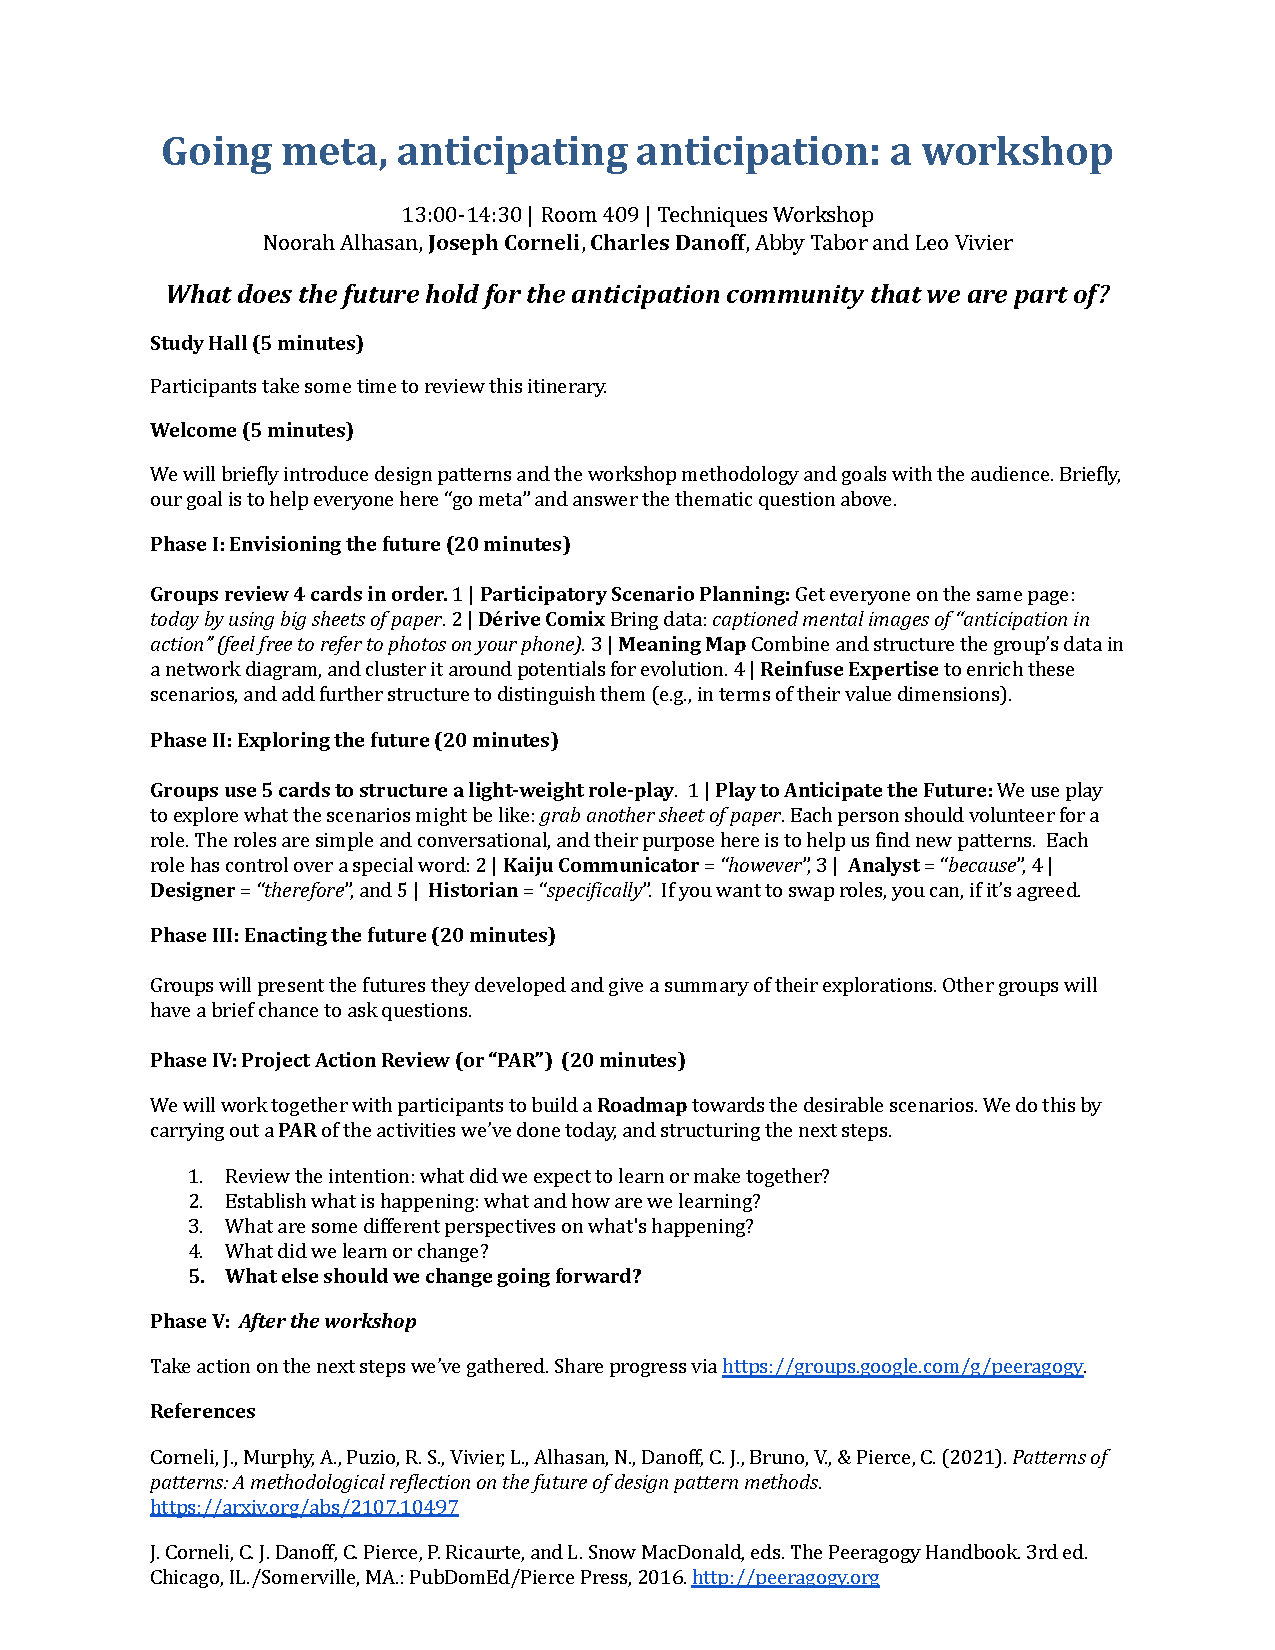
\includegraphics[width=\textwidth,trim={1cm 4.5cm 1cm 4.5cm},clip=true]{anticipation}
\end{mdframed}

\clearpage

\subsection{Intermediate artifacts}

\begin{figure}[h]
\begin{tabular}{c@{\hspace{1em}}c}
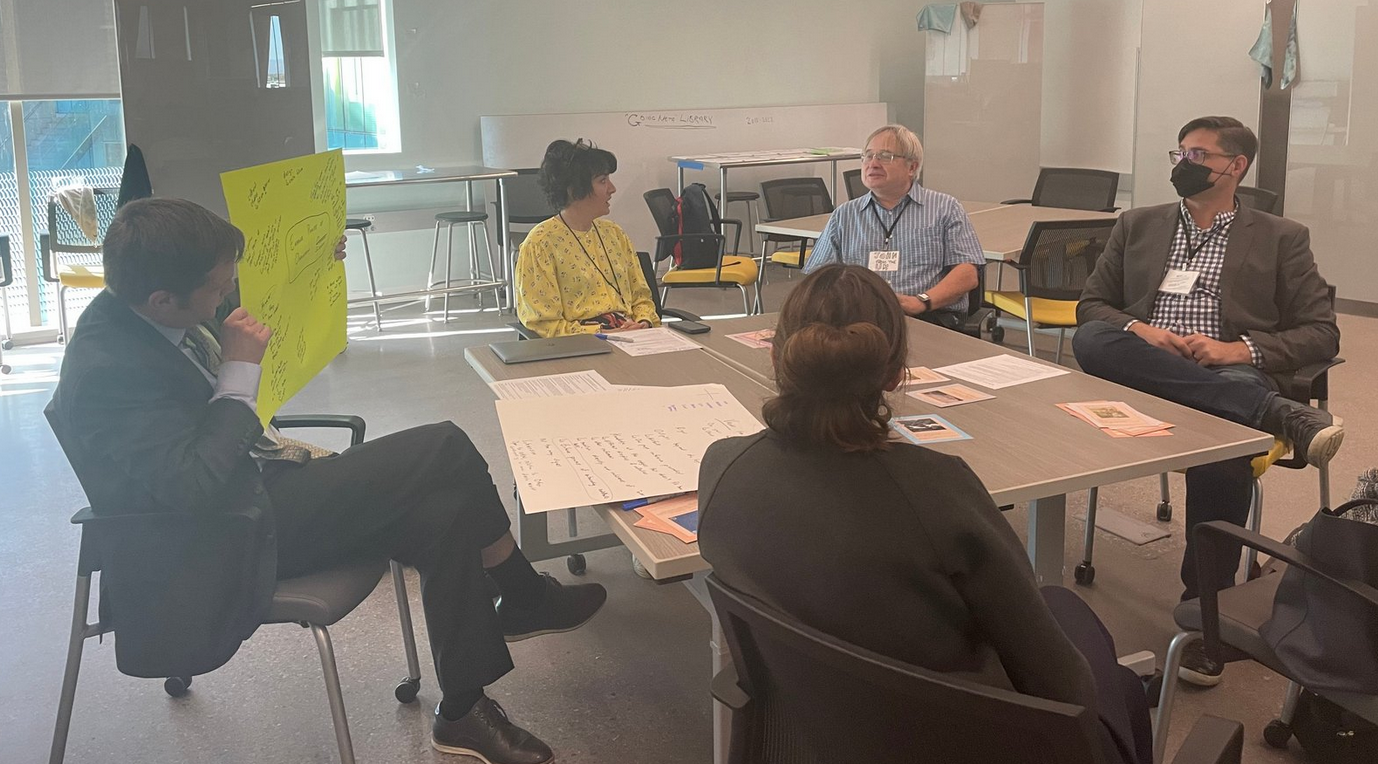
\includegraphics[width=.45\textwidth]{AnticpationWorkshop.png}  &
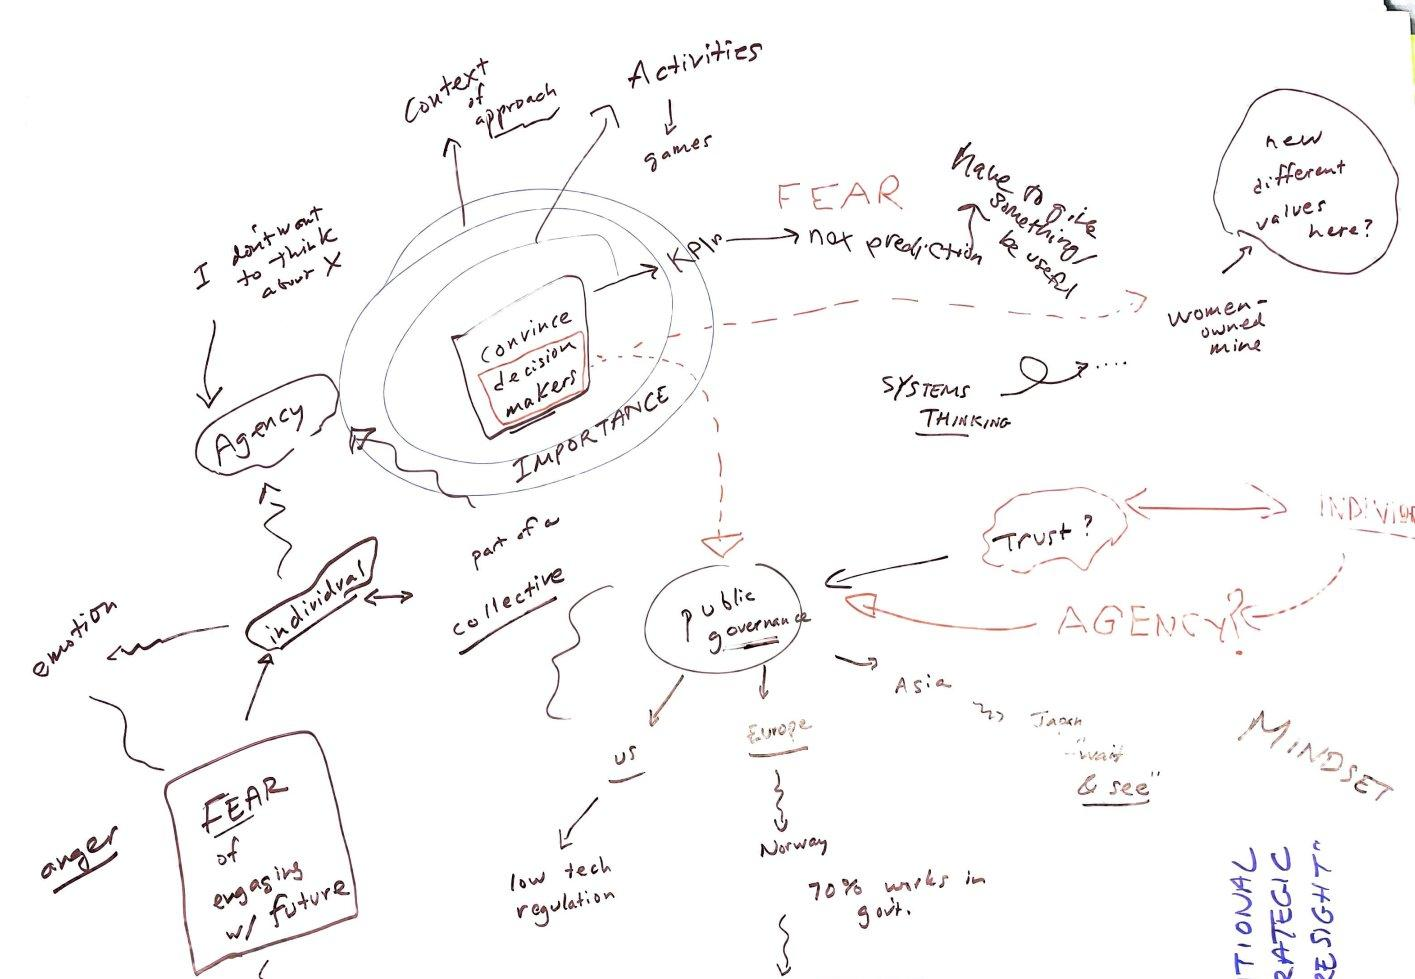
\includegraphics[width=.45\textwidth]{Anticipation-Mindmap.jpeg}
\end{tabular}
\caption{In the workshop, participants used cards to structure discussions, and facilitators took notes and made diagrams.\label{anticipation-workshop}}
\end{figure}

\noindent
Figure \ref{anticipation-workshop} shows the workshop in process
(left) and details of the notes taken by one of the facilitators
(right).  Facilitators moved between facilitating small-group and
whole-group activities.  In the ``Phase IV'' review, participants had
different responses to our request to reflect on the workshop’s
activities.  Some considered the workshop to have led to good
conversations, but doubted if the manipulatives and other structures
helped.  However, we observed that some participants had used the
manipulatives in creative ways—such as asking each other to pass
around the cards to better narrate the points they were making in the
conversation.  (This experience highlights the ‘motor’ aspect of the
{\sc Functional Roles}!)  No new design patterns were generated on the
day, but follow-up reflections on the experience did suggest some
patterns.

\subsection{Output patterns}

\emph{The framing of our workshop relative to the Anticipation
conference suggests a repeatable pattern:}

\subsection*{GOING META{\hfill (c)}}\label{method1}
\label{sec:org958ff04}

\textbf{Context} In the course of working on a project
together.\newline \textbf{If} we find a \textit{gap} between our
ideals and our methods;\newline \textbf{Then} Try “going meta”, to
explore how the project’s methods can be applied to itself.\newline
\textbf{Example} In a community that usually focuses on anticipating
the future for others, try inviting members of the community to
anticipate the future of the community.


\medskip

\noindent \emph{Reflecting on the attendees’ contributions, both in
terms of their concrete comments about the Anticipation community as
well as the way they interacted within the workshop (e.g., by
contributing to note-taking and by leading conversations as the
facilitators moved around the room) gave rise to the following
proto-pattern:}

\subsection*{💎 INCREASE PARTICIPANT CONTROL {\hfill \motor}}

When organising a collaborative activity, participants should not
remain only an audience, or only deliver scripted lines.  Give them
increasing responsibility.


\medskip

\noindent \emph{Looking back at some remove, we can also notice a
pattern that relates the work in this section to the paper:}

\subsection*{💎 PILOT TO ANTICIPATE {\hfill \sensory}}

Invoking the {\sc Going Meta} pattern, we reflect that our strategy of
\emph{piloting our workshop methods} was how we choose to anticipate
the issues likely to arise in future iterations of the workshop.
Perhaps the future of anticipation more widely will include the
increased use of pilot schemes?  In support of this possibility \citet{unger2019imagination} have advocated for the enthusiastic embrace of “Experimental government”.


\subsection{Diagrammatic summary of the “PLACARD” process (and the “Open Future Design Workshop”)}\label{illustrative_diagram}
The diagram in Figure \ref{alex-diagram} shows how the new patterns
like {\sc Going Meta} and {\sc Increase Participant Control} would be
synthesized by following the PLACARD method, enlarging the “Pattern
space” within a given domain.  Notice that the “Going Meta” deployment
of Open Future Design at Anticipation 2022 made explicit use of DPL
and PAR, while only touching briefly on CLA.  However, all three of
the sensory, cognitive, and motor dimensions of PLACARD were brought
into play with the patterns {\sc Dérive Comix}, {\sc Meaning Map}, and
{\sc Functional Roles}.

\begin{figure}[h!]
  %  \includegraphics[width=.8\textwidth,page=3,trim={2cm 8.5cm 1.6cm 2cm},clip=true]{alex_thoughts}
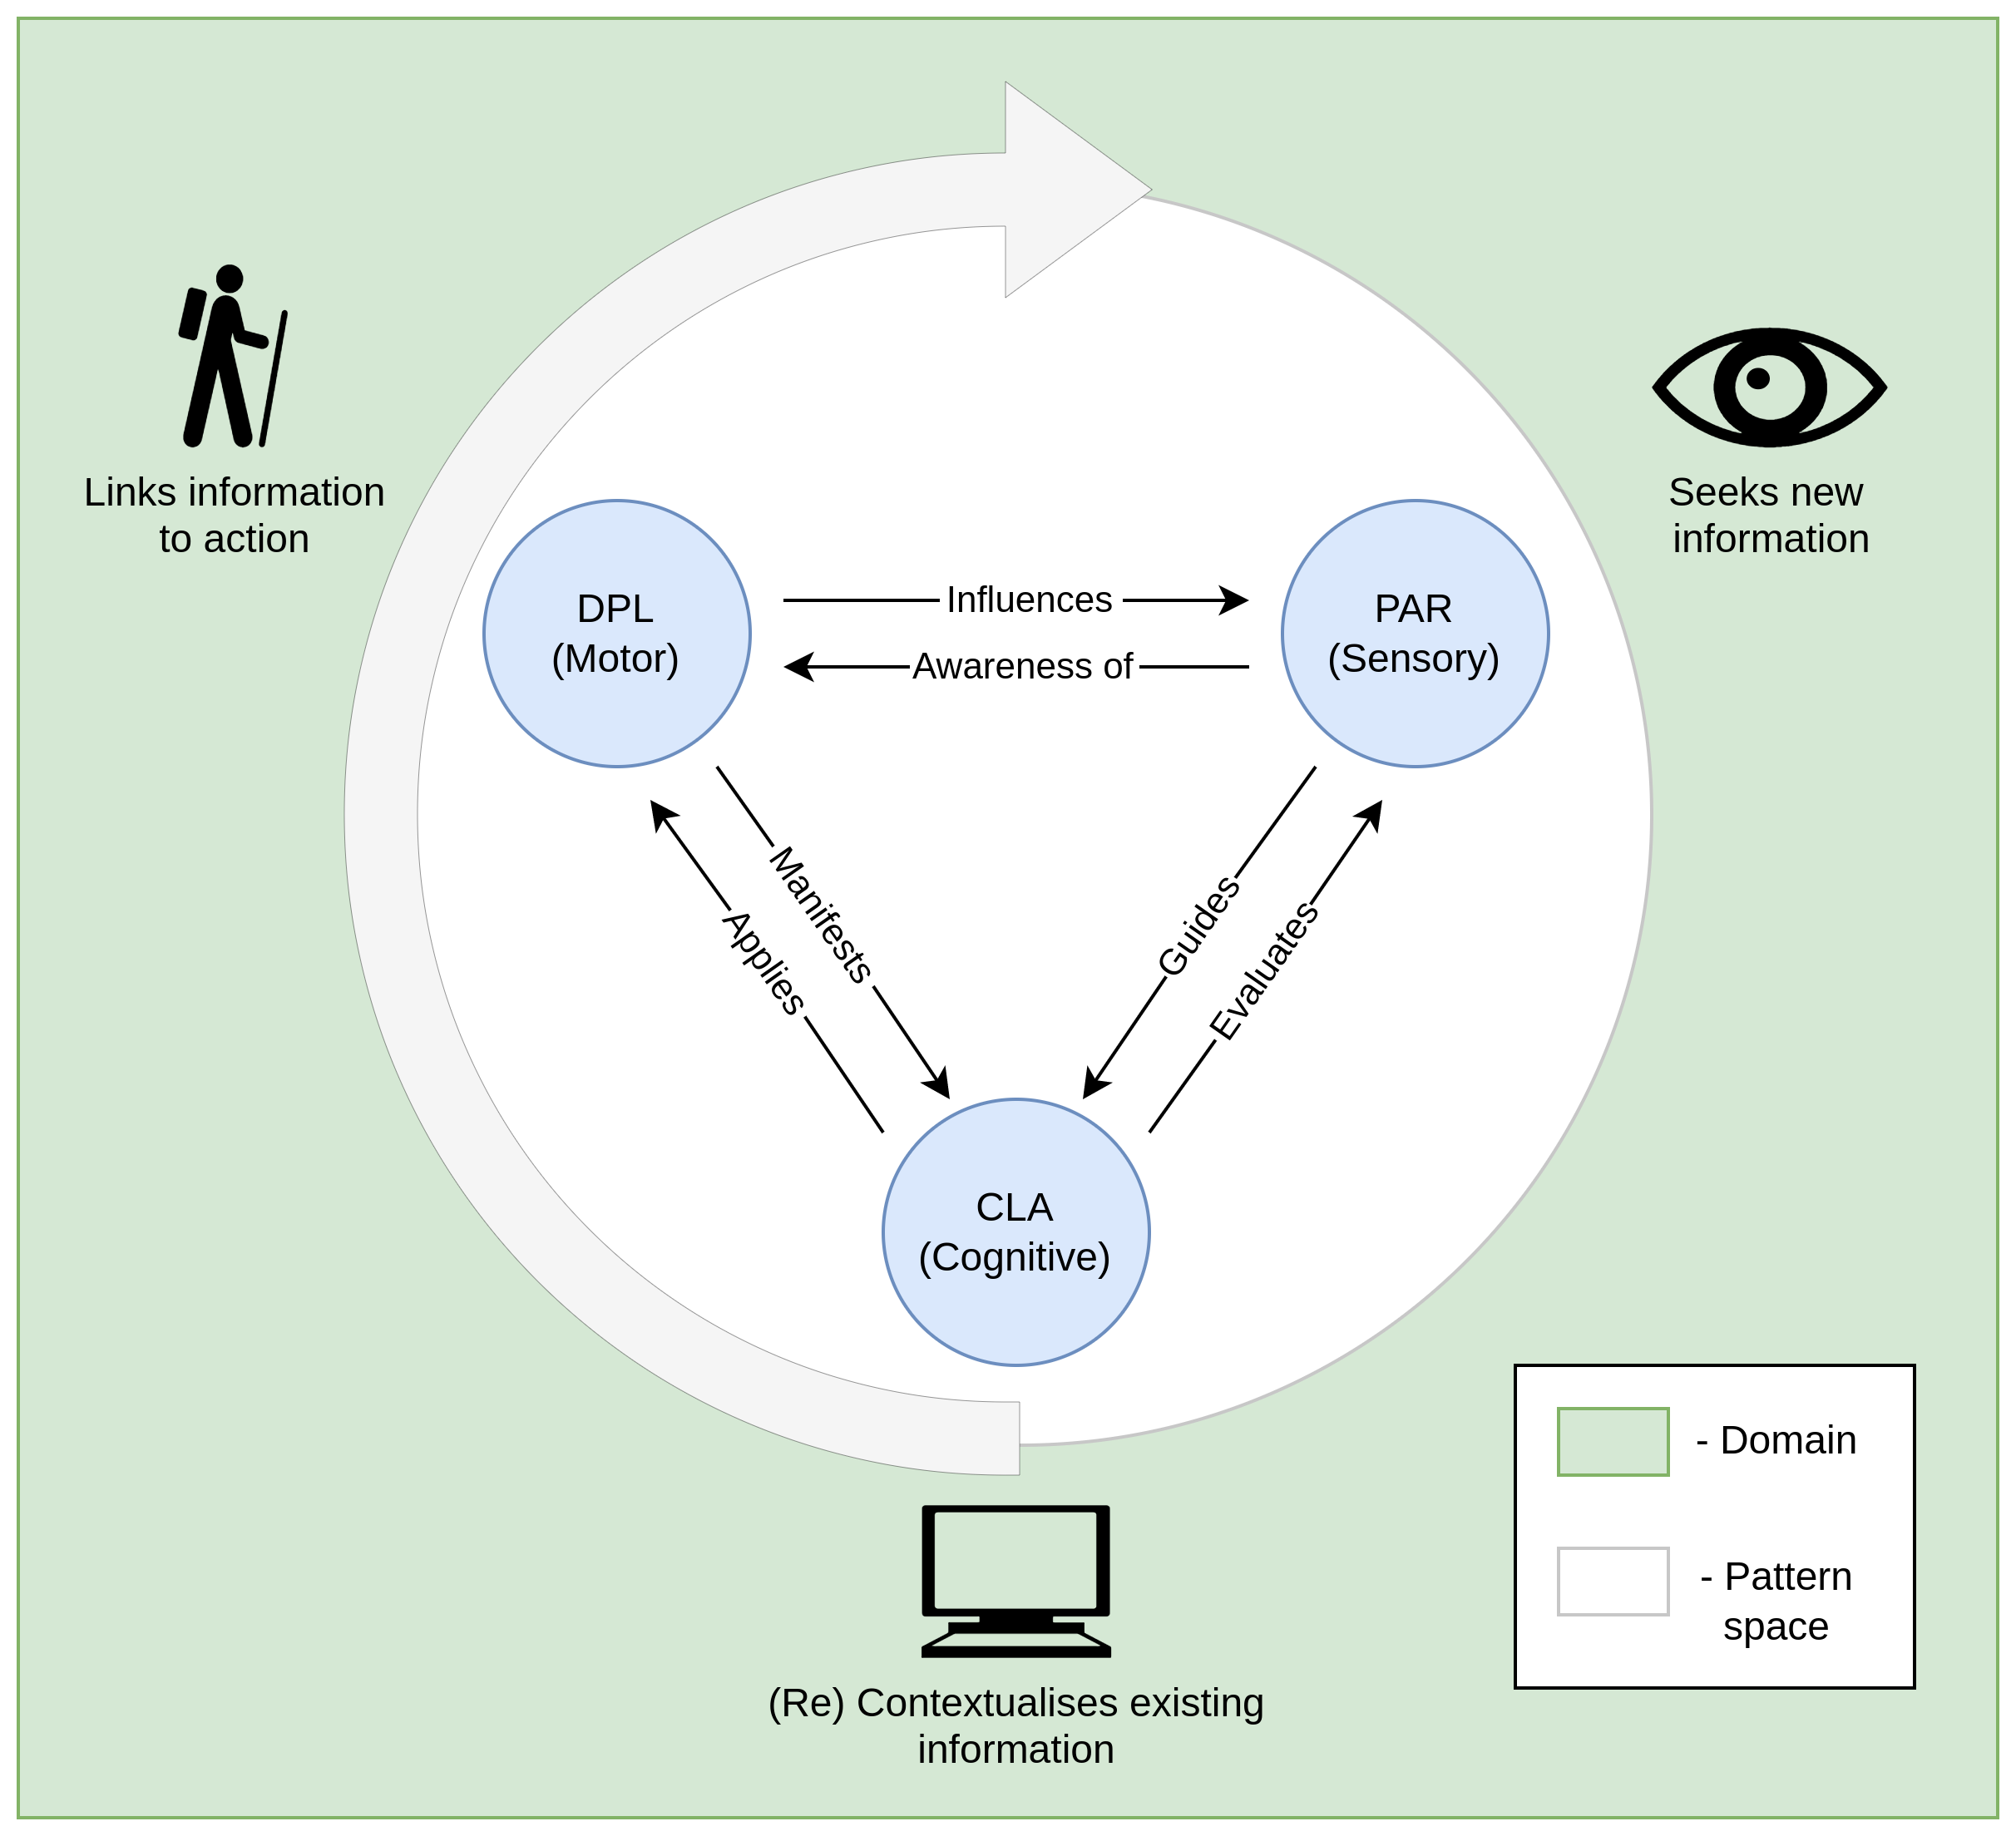
\includegraphics[width=.8\textwidth]{alex-image-updated.png}
  \caption{Relationships between sensory, cognitive, and motor patterns (paralleling {\scitshape MB Drawing a Map} from \citet{iba2016pattern}), here illustrating the potential for the space of patterns to grow as these methods are applied within a domain.\label{alex-diagram}}
\end{figure}

\clearpage

\section{Case Study 2: Public Space for Public Health}\label{second-case-study}

This workshop was commissioned by co-author Abby Tabor as part of her
research project at the University of the West of England on
“Designing urban environments for human health: from the microbiome to
the metropolis”.  The aim was to gather attendees with an interest in
the project themes and work together to envision next
steps. Elaborations of these were developed by participants, and were
organized by facilitators using a software tool based on Org Roam and
Org Roam UI.
% \footnote{Demo: \url{https://hyperreal.enterprises/bristol}}

Alongside the patterns from our Anticipation pilot, here looked for
new methods to {\sc Increase Participant Control}.  In particular, we
generated some further articulations of the {\sc Functional Roles}
that would help with this.  The roles presented come with mnemonic
symbols based on the chess set: at the workshop, participants were
provided with additional physical manipulatives, i.e., the chess
pieces that correspond to the symbols here, along with new pattern
cards similar to those in Figure \ref{cards}, featuring the
descriptions here.  As mentioned previously, in the Anticipation
pilot, the roles were aligned with the {\sc Pattern Language
  Components}.  For example, previously the “{\sc Kaij\=u
  Communicator}” role (here, renamed and adapted as the “{\sc
  Wrinkler}”) had final say over the challenges implied by the
‘however’ keyword.  In still-earlier pilots, the roles were assigned
more elaborate responsibilities, and participants would receive a
brief training for the role prior to taking it on.  For example, the
{\sc Designer} role (now dropped entirely) was briefed on a specific
collection of design patterns.

As presented in this workshop, the roles were strictly functional and
were not the focus of role play as such.  Rather, an attendee would
fill a given role momentarily within a conversation, while remaining
fully themselves.

\subsection{Input patterns}

\emph{Alongside the descriptions of the roles that were given to
participants (again with pattern cards), the reader may refer to Table
\ref{mnemonic-for-manipulatives} which explains the mnemonic meaning
of the chess pieces which accompanied each role description.  A
similar informal description of the roles was also given to
participants.}

\begin{table}[h]
\begin{tabular}{llp{.5\textwidth}}
\textbf{Role} & \textbf{Manipulative(s)} & \textbf{Explanation}\\ {\sc
  Time Traveler} & {\chess ♕} & In chess, the Queen can move linearly
in any direction: forward, backward, and diagonally.  Similarly, the
{\sc Time Traveler} role ‘moves’ both backwards and forwards in time,
and also explores the conditions that appear at those points in
time.\\

{\sc  Analyst} & {\chess ♗}, {\chess ♝} & In chess, there are two Bishops, both of which move diagonally, so that both are restricted to different colored squares. Here the {\sc Analyst} role divides its attention across two different spheres: articulations within the current challenge, and articulations of this challenge relative to other challenges.  \\

{\sc Wrinkler} &  {\chess ♘} & In chess, the Knight moves in a skewed fashion: in order to go in one direction, it must also go a little bit in another direction.  The {\sc Wrinkler} role, similarly, looks at how a given strategy might go askew, due to unintended consequences or otherwise.\\

{\sc Linker} &  {\chess ♖} & In chess, the Rook moves any distance, as long as it goes in a straicoght line.  The {\sc Linker} role, similarly, can record a link between any two related concepts.  Since all concepts are potentially related in some fashion, the {\sc Linker} focuses on making \emph{useful} connections.\\

{\sc Reflector} &  {\chess ♔} & In chess, capturing the King means the end of the game, so players are concerned throughout with any threat to their King.  Here, the {\sc Reflector} role senses how the discussion of a given scenario is progressing and when it would be good to draw it to a close and move on. 
\end{tabular}
\caption{Mnemonic for manipulatives based on the chess set\label{mnemonic-for-manipulatives}}
\end{table}


\subsection*{TIME TRAVELER {\chess ♕} {\hfill \sensory}}

\textbf{Question} \emph{What has happened in the past, what could
happen in the future?}\newline
\textbf{Role} To provide historical context and
anticipate alternate futures.


\subsection*{WRINKLER {\chess ♘} {\hfill \motor}}

\textbf{Question} \emph{What could go wrong? }\newline
\textbf{Role.} Consider what might derail or counter
the proposed solution.  Each wrinkle can be assigned a level of
perturbation (from low to high).


\subsection*{ANALYST {\chess ♗♝} {\hfill \cognitive}}

\textbf{Question} \emph{What are the moving parts?}\newline
\textbf{Role 1} Consider the current challenge and all the components
of the potential solution (actors, resources, institutions). Identify
and orchestrate the dynamic network of these components.\newline
\textbf{Role 2} Consider the other challenges specified beyond the
current focus.  Identify and orchestrate the integration of these
components relevant to the present challenge.


%\textbf{Example} Everyday roadmap languages include both iconic map and road sign symbols; when people are confused or lost they may ask for help or try to find their own way back to the road using other informal languages.

\smallskip

\noindent \emph{(We also characterized some roles which would be
filled by offsite and onsite facilitators.)}

\subsection*{FACILITATOR ROLES {\hfill \cognitive}}
\textbf{Context} Developing a collection of interrelated design
patterns.\newline \textbf{If} you are getting ideas from participants
who play {\sc Functional Roles} BUT the ideas aren’t all connected
with each other in a structured way.\newline \textbf{Then} introduce
facilitator roles to help structure the collection.\newline
\textbf{Specifically}, {\sc Linker}s, and {\sc Reflector}s are two
roles that we have found useful.


\smallskip \noindent \emph{The following patterns describe specific
functions which were filled by offsite and onsite facilitators.}

\subsection*{LINKER {\chess ♖}{\hfill \cognitive}}

\textbf{Question}
\emph{How do proposed scenarios build into patterns across layers, and how do they interact within the constellation of related concepts?}\newline
\textbf{Role.} Data wrangling as it comes in, providing visualization of patterns and interconnections.


\subsection*{REFLECTOR {\chess ♔}{\hfill \sensory}}

\textbf{Question} \emph{How is the scenario evolving?}\newline
\textbf{Role} To appraise each developing scenario, provide a format
for reflection (e.g., PAR), make a decision to continue, reset, or end.


\smallskip \noindent\emph{In the spirit of {\sc Increasing Participant
  Control}, the {\sc Facilitator roles} could be distributed to
participants, though doing so in a future workshop would require
spending more time on training, and potentially also improved
tooling.}

\clearpage
\subsection{Itinerary}

\begin{mdframed}[backgroundcolor=blue!50,linecolor=blue!50]
  \noindent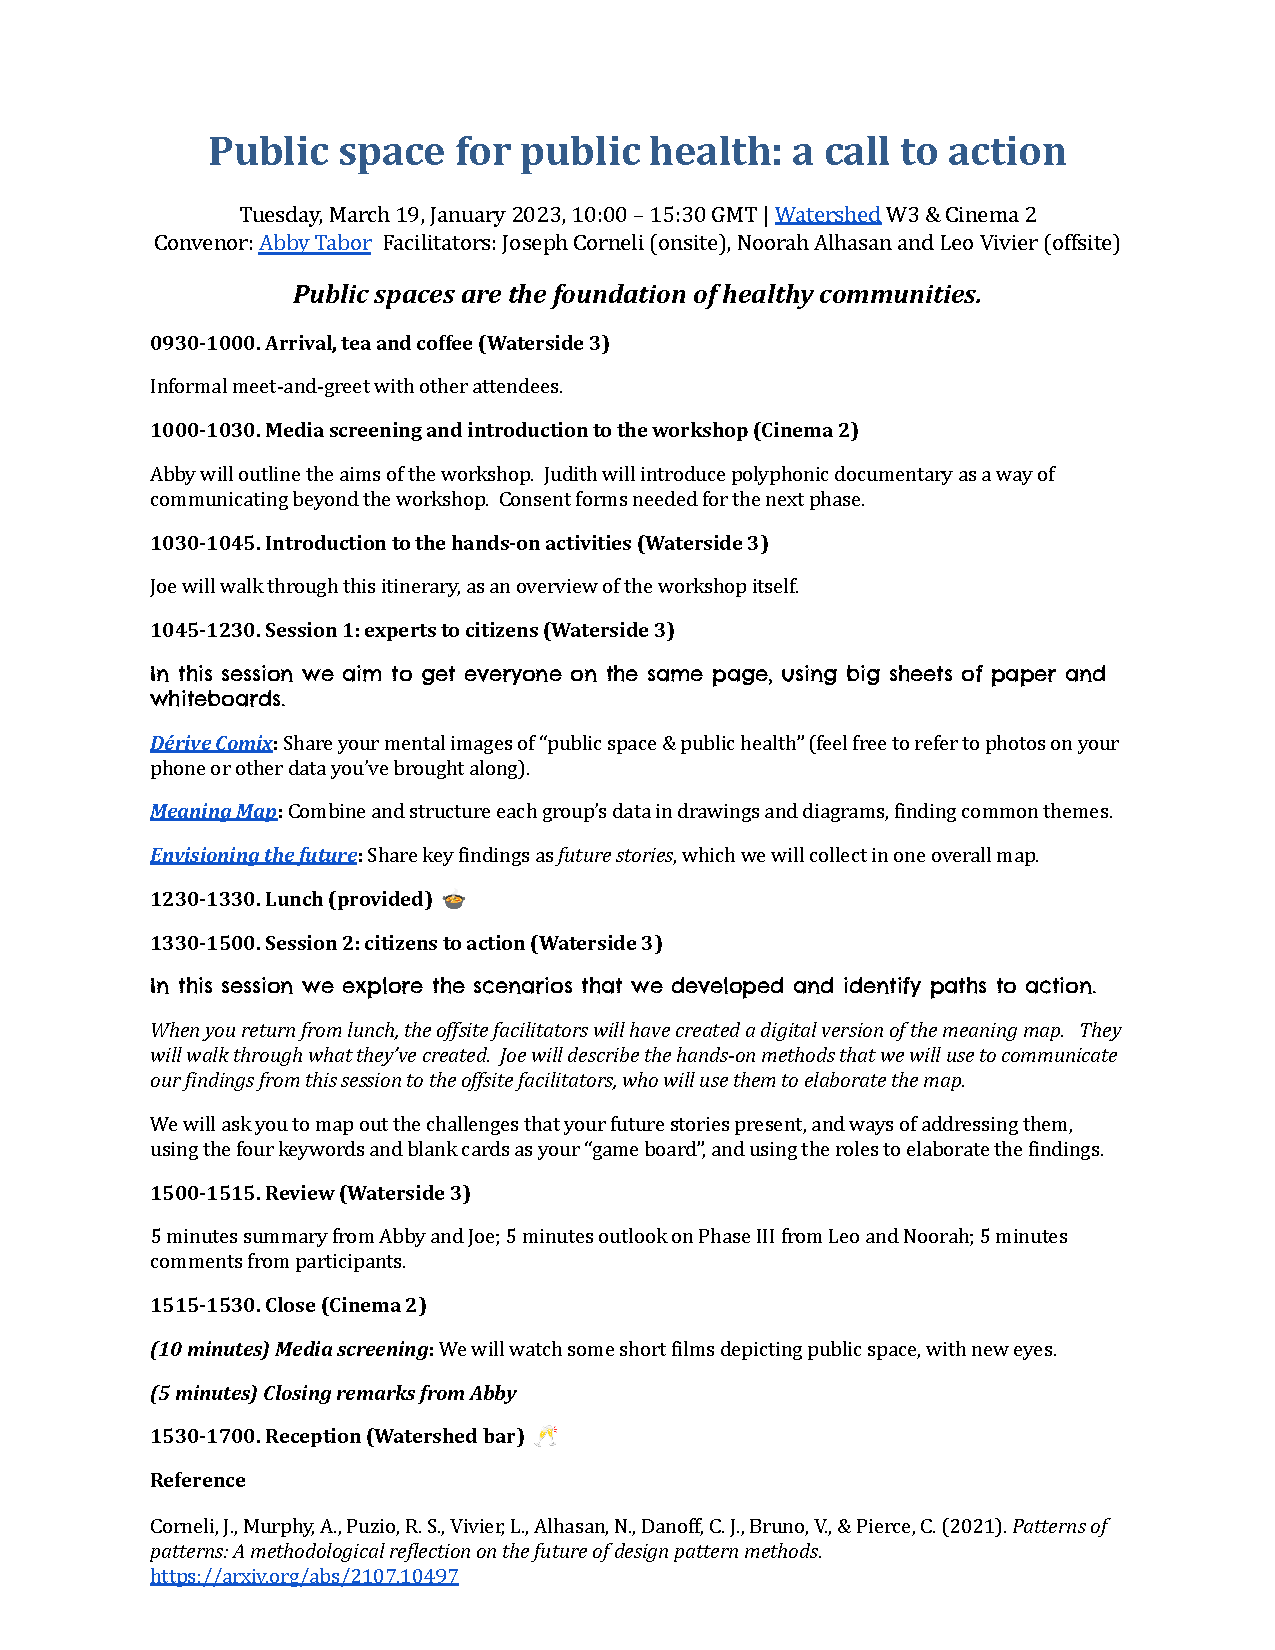
\includegraphics[width=\textwidth,trim={1cm 3.2cm 1cm 4.5cm},clip=true]{bristol}
\end{mdframed}

\subsection{Intermediate artifacts}

Intermediate artifacts generated within the workshop included mindmaps
created with participants, on paper.  We used a graphical template
following the outline of the Causal Layered Analysis layers to explain
the workshop’s overall workflow, and also asked participants to use a
version of this diagram as a “grid” for note-taking within Phase I, to
encourage them to work from their observations to the core underlying
themes and issues.  Participants then clarified these core themes in a
share-back process, and in Phase II, developed them further in the
form of shared future stories, outlining paths to action.  Photos in
Figure \ref{ExampleParticipantPattern} show the movement from:
\begin{itemize}
  \item Initial sketching at the start of Phase I, beginning at the
    \emph{litany} level, within small groups, to:
  \item A collection of themes shared across groups at the end of
    Phase I, to create a {\sc Meaning Map} which, in CLA terms, is
    intended to bring everyone into a shared \emph{myth} layer, on to:
  \item Phase II work using {\sc Pattern Language Components}, to
    identify both general and specific possibilities for action around
    a theme.
\end{itemize}

\begin{figure}
  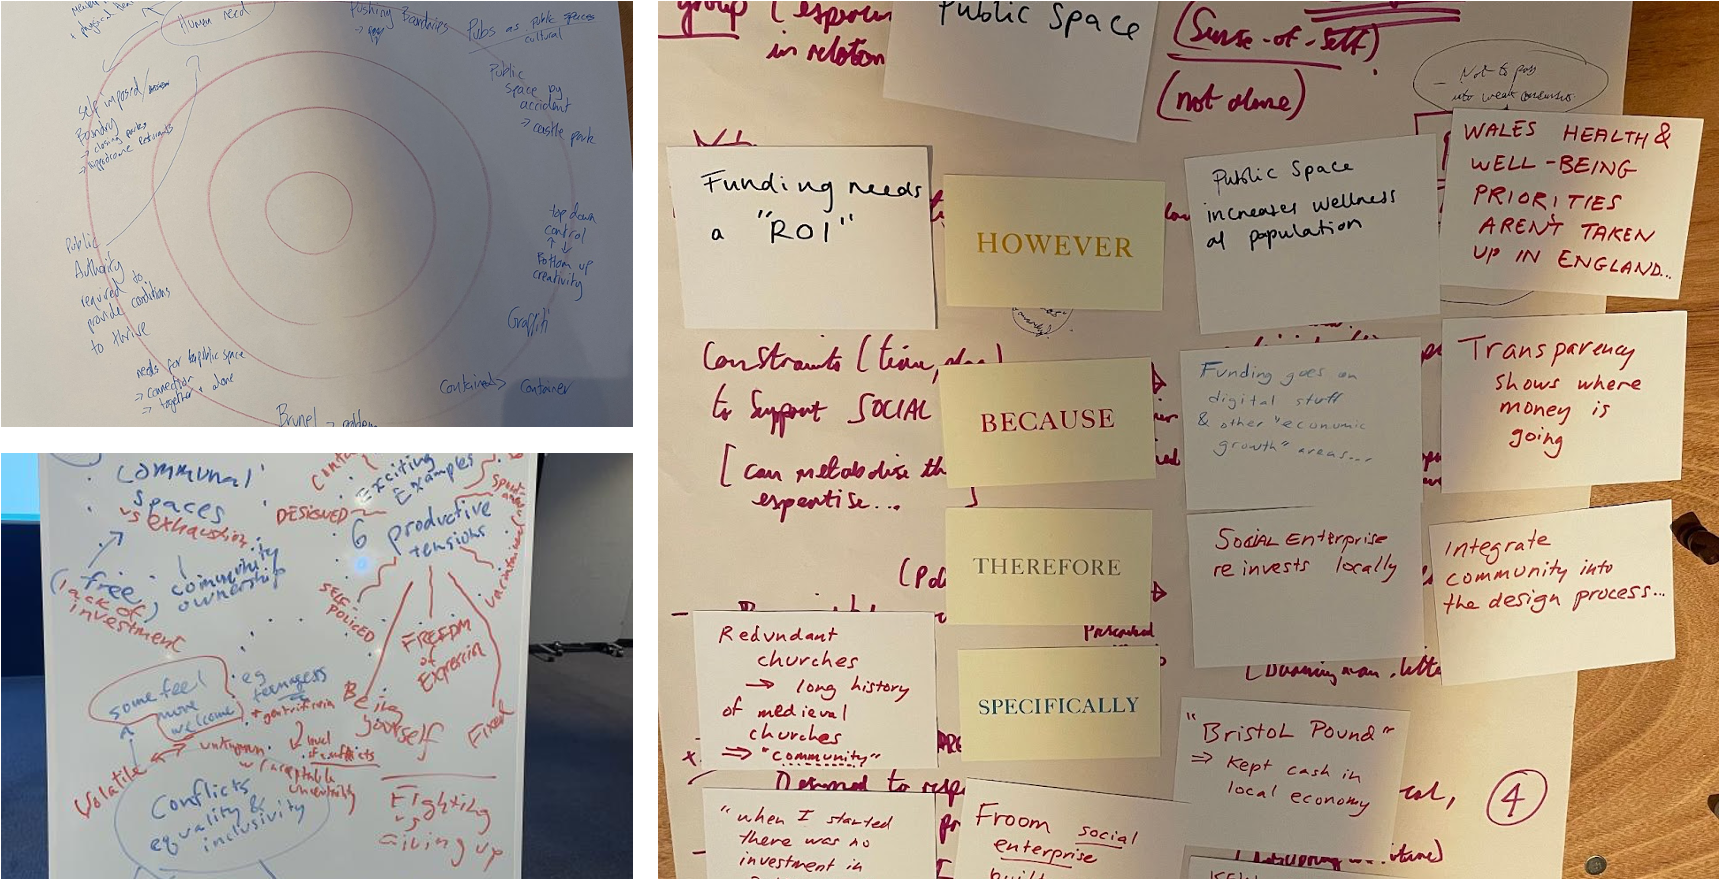
\includegraphics[width=\textwidth]{PatternProcess.png}
  \caption{Use of diagrams and manipulatives to create meaning maps
    and new patterns (paralleling {\scitshape MA 1.3 Mining
      Atmosphere} from \citet{iba2016pattern}. In the upper-left
    photo, the CLA layers are mapped to concentric circles; from
    outside to center: litany, system, worldview, myth.  The {\sc
      Share Back} pattern was used to collect core themes from groups
    working separately, as the basis of a shared myth (lower left).
    {\sc Pattern Language Components} were used to sketch solution
    strategies to key problems and concerns, e.g., {\sc Funding of
      Public Space} (right). \label{ExampleParticipantPattern}}
\end{figure}

\clearpage

\subsection{Output patterns} \emph{Participants created several patterns by making use of
the {\sc Pattern Language Components} and {\sc Functional Roles}.
Here, the material shared by participants is summarized and condensed
in proto-pattern form.  For an example showing how the patterns looked
in the workshop, see the right-most image in Figure
\ref{ExampleParticipantPattern}, which details the participants’
articulation of the {\sc Funding of Public Space} pattern (with help
from a workshop facilitator).}

\subsection*{\normalsize{\emoji{pick}\emoji{gem}} CONTESTED SPACE{\hfill \sensory}}\label{pat:contested-space}

So-called public space doesn’t always feel welcoming to all members of the public.  It can be overrun with antisocial behavior.  It can feel exclusionary, or uninviting.  It can be the site of conflict.  Although the uses of public space are complex, each space need not support every use equally.


\subsection*{⚒💎 REBALANCE SOCIAL SERVICES{\hfill \motor}}\label{pat:rebalance-social-services}

Welfare-related services should be supplied in balance with local needs, though they often are not. Can varied expertise be integrated in a similar way to the domain-specific skills practiced by Médicins Sans Frontièrs to address complex local challenges?


\subsection*{\normalsize{\emoji{pick}\emoji{gem}} FUNDING OF PUBLIC SPACE{\hfill \cognitive}}\label{pat:funding-of-public-space}

Even though public space is known to increase wellness in the
population, well-being priorities that would lead to increased funding
for public space aren’t universally adopted.  In order to make the
benefits of such investment clear, increase transparency around
investments in public welfare, e.g., create a register of impacts of
local social enterprises.


\smallskip
\noindent \emph{Reflecting on the contributions of Abby Tabor as
workshop convenor, and special guest Judith Aston who framed our
activities in relation to broader ‘interactive documentary’ practices
\cite{Aston2017}, we can observe a simple pattern that would be useful
in subsequent workshops.}

\subsection*{CONTEXT SETTING {\hfill \sensory}}
\textbf{Context} A workshop or other working context has been
convened.\newline \textbf{If} the facilitators have ideas that they
would like to explore with attendees BUT these ideas are not top of
mind for attendees.\newline \textbf{Then} do some context-setting,
e.g., showing videos, giving a short talk about why people have been
invited and describe the hoped-for outcomes.


\smallskip
\noindent \emph{With hindsight, another role comes to mind, which was
not explicitly presented in the workshop, but which echoes our overall
aim to identify possible paths to action.  The {\sc Stepper} role
harkens back to the use of “next steps” together with patterns,
introduced in \citet{corneli2015a}.  Table \ref{mnemonic-for-stepper}
supplements Table \ref{mnemonic-for-manipulatives} with a description
of the corresponding mnemonic.}

\begin{table}[h]
\begin{tabular}{llp{.5\textwidth}}
\textbf{Role} & \textbf{Manipulative} & \textbf{Explanation}\\ {\sc Stepper} &  {\chess ♙} & In chess, Pawns move one space at a time (or two at the beginning of their movement).  Pawn are individually weak, but collectively, their placement is important for strategy.  The {\sc Stepper} role similarly describes the immediate next actions that should be taken at a point in time.
\end{tabular}
\caption{Mnemonic for the {\sc Stepper} role \label{mnemonic-for-stepper}}
\end{table}

\subsection*{STEPPER {\chess ♙} {\hfill \motor}}

\textbf{Question} \emph{What should we do next?}\newline \textbf{Role}
Consider the discussion so far, and the various possibilities for
action that have arisen.  Decide which actions would be most useful or
informative, and devise a plan in place to carry them out.\newline


\noindent \emph{A related ambition, which we did not realize within
the scope of this project, was the creation of a wiki, which would
have been a place to collect next steps, and share updates and
reportage on collaborative work around the possible actions surfaced
during the workshop.  Instead, the notes taken by off-site
facilitators were presented back to participants in a (non-editable)
wiki-like prototype. Cf. Case Study 3 for further details of a related
prototype.}

\subsection{Further remark on the Roles of Roles}\label{role-of-roles}
Relevant high-level next steps following up on this workshop would be
revise and re-articulate the proto-patterns above in more formal
terms, alongside a process of evidence-gathering that would support or
refute the value of specific interventions which ramify the patterns
in their local context.  These future operations might be supported by
new {\sc Functional Roles}, or by further elaborations of those
already described above.  Indeed, review (e.g., during a PAR) of the
contributions to the process that were made by different roles could
help to articulate the need and plan for evolution at the process
level.  Presently, with Table \ref{active-inference-factors} we draw
attention to the way in which the participant roles outlined above
operationalize key aspects of the Active Inference Framework (see
\citet{SMITH2022102632} for a primer on the key concepts in AIF).
%% It might integrate
%% something like our {\sc Functional Roles} roles into patterns
%% themselves, so that a pattern or pattern language would be able to
%% ‘sense’ when it needs to be revised or elaborated.

% Change table rules to add .2em vertical space for easier reading LEO

{
\renewcommand*{\arraystretch}{1.2}
\begin{table}[h]
\begin{tabular}{rp{.5\textwidth}}
{\sc Time Traveler} & contributes to elaborating \emph{the prior
belief over states} and the \emph{likelihood of specific
observations}.\\

{\sc  Analyst} & contributes to elaborating the \emph{generative model}, with the division between inward and outward articulations corresponding to \emph{internal} and \emph{external}-facing (i.e., \emph{sensory} and \emph{active}) states.\\

{\sc Wrinkler} & contributes to elaborating the \emph{factor of surprisal}.\\
{\sc Stepper} & takes action to correct discrepancies between the generative model and the perceived state of the world, minimizing \emph{prediction error}.
\end{tabular}
\caption{Key factors in the Active Inference Framework are reflected in participant roles\label{active-inference-factors}}
\end{table}
}

Active Inference is currently being explored as a new paradigm for
artificial intelligence
\cite{friston2022designing,albarracin2023designing}.  Here, we suggest
that AIF and DPL can support each other, with AIF concepts being given
a practical implementation using design pattern methods, and DPL
receiving a needed theoretical upgrade from Active Inference.  The
{\sc Functional Roles} in Table \ref{active-inference-factors} focus
on the generation of next steps.  Another notable commonality between
DPL and AIF is that both typically make use of hierarchically
organization, e.g., \emph{A Pattern Language} zooms in from patterns
for towns to buildings to construction; whereas AIF zooms out, from “I
model the world” to “we model the world” to “we model ourselves
modelling the world” \cite{Kirchhoff2018}.

This suggests further strategies for building structured approaches to
complexity.  For example, \citet{benoit2019structure} paraphrase
Christopher Alexander’s conception of urban development: “‘natural’
cities evolve by maintaining their amount of surprisal constant on
average.”  Further elaboration and orchestration of {\sc Functional
  Roles} could provide similar guidelines for the evolution of pattern
languages, helping to ameliorate the structural limitations of pattern
language development, such as those described by \citet{Dawes2018}.


% building on these descriptions, and which would help to express the
% strategic role of the various constituent patterns.

\clearpage
\section{Case Study 3: Open Research Futures}

This workshop was developed as an “Away Day” for faculty and staff
members at Oxford Brookes University.  The aim of the workshop is to
elaborate the institution’s open research strategy relative to its
existing organizational strategy.  Methodologically, this workshop
builds on a pre-seeded Org Roam network of interlinked themes and an
additional activity that enlists attendees in taking concrete actions
on the identified next steps.  This itinerary reused the language
“experts to citizens”, “citizens to action” from the previous workshop
(with a slight variation suited to the context).  It is worth
remarking here that these phases mirror the {\sc Dérive Comix}—{\sc
  Meaning Map}—{\sc Reinfuse Expertise} structure introduced in the
first case study, and that, in CLA terms, the effect is a journey from
\emph{litany-to-myth-back-to-litany}, with the new litany taking the
form of potential actions.

\subsection{Input Patterns}

\subsection*{DO YOUR RESEARCH{\hfill\sensory}}
\textbf{Context} Prior to beginning a formal workshop or other participatory research activity.\newline
\textbf{If} it looks like it will be possible to do participatory research BUT the participants haven’t begun speaking with each other yet.\newline \textbf{Then}
start doing the research in a more centralised way before inviting direct collaboration, in order to give participants something to engage with.\newline
\textbf{Example} In the current setting, this pre-research included 1-to-1 interviews with about half of the invitees, as well as internet research to find and explore related scenarios developed by others.\footnote{\url{https://royalsociety.org/topics-policy/projects/research-culture/changing-expectations/visions-of-2035/visions-of-2035-materials/}}


\subsection*{STRUCTURE CONVERSATIONS{\hfill\cognitive}}
\textbf{Context} Having convened a workshop or other participatory research activity.\newline
\textbf{If} unstructured discussions are likely to take lots of time but without yielding concrete benefits.\newline \textbf{Then}
structure the discussions around shared interests to move things forward more effectively.\newline
\textbf{Example} At this workshop, we decided to group participants around tables according to the faculty where they were employed (or most closely aligned, in the case of university-level support staff).


\subsection*{THE FUTURE BEGINS NOW{\hfill\motor}}
\textbf{Context} Having developed possible next steps in a discussion.\newline
\textbf{If} it appears that leaving the discussion without concrete commitments means concrete actions are less likely to take place.\newline \textbf{Then} take preliminary actions before leaving the discussion to create a sense of commitment and follow-through.\newline
\textbf{Example} One way to build commitment would be to ask people to develop and share a method for a small-scale experiment that they plan to carry out.


\smallskip
\noindent \emph{In the event, there was not enough time to do the
activities described in {\sc The Future Begins Now} within this
iteration of the workshop.  One possible reason for this is that the
{\sc Stepper} role, introduced in the commentary in Case Study 2, had
not been conceptualised, and handed out to participants in this
workshop.  So, even though participants were invited to think about
potential next steps using the \emph{SPECIFICALLY} keyword from the
{\sc Pattern Language Components} pattern, there wasn’t a
corresponding {\sc Functional Role} which would help participants
“own” those steps.}
\clearpage

\subsection{Itinerary}

\begin{mdframed}[backgroundcolor=blue!50,linecolor=blue!50]
  \noindent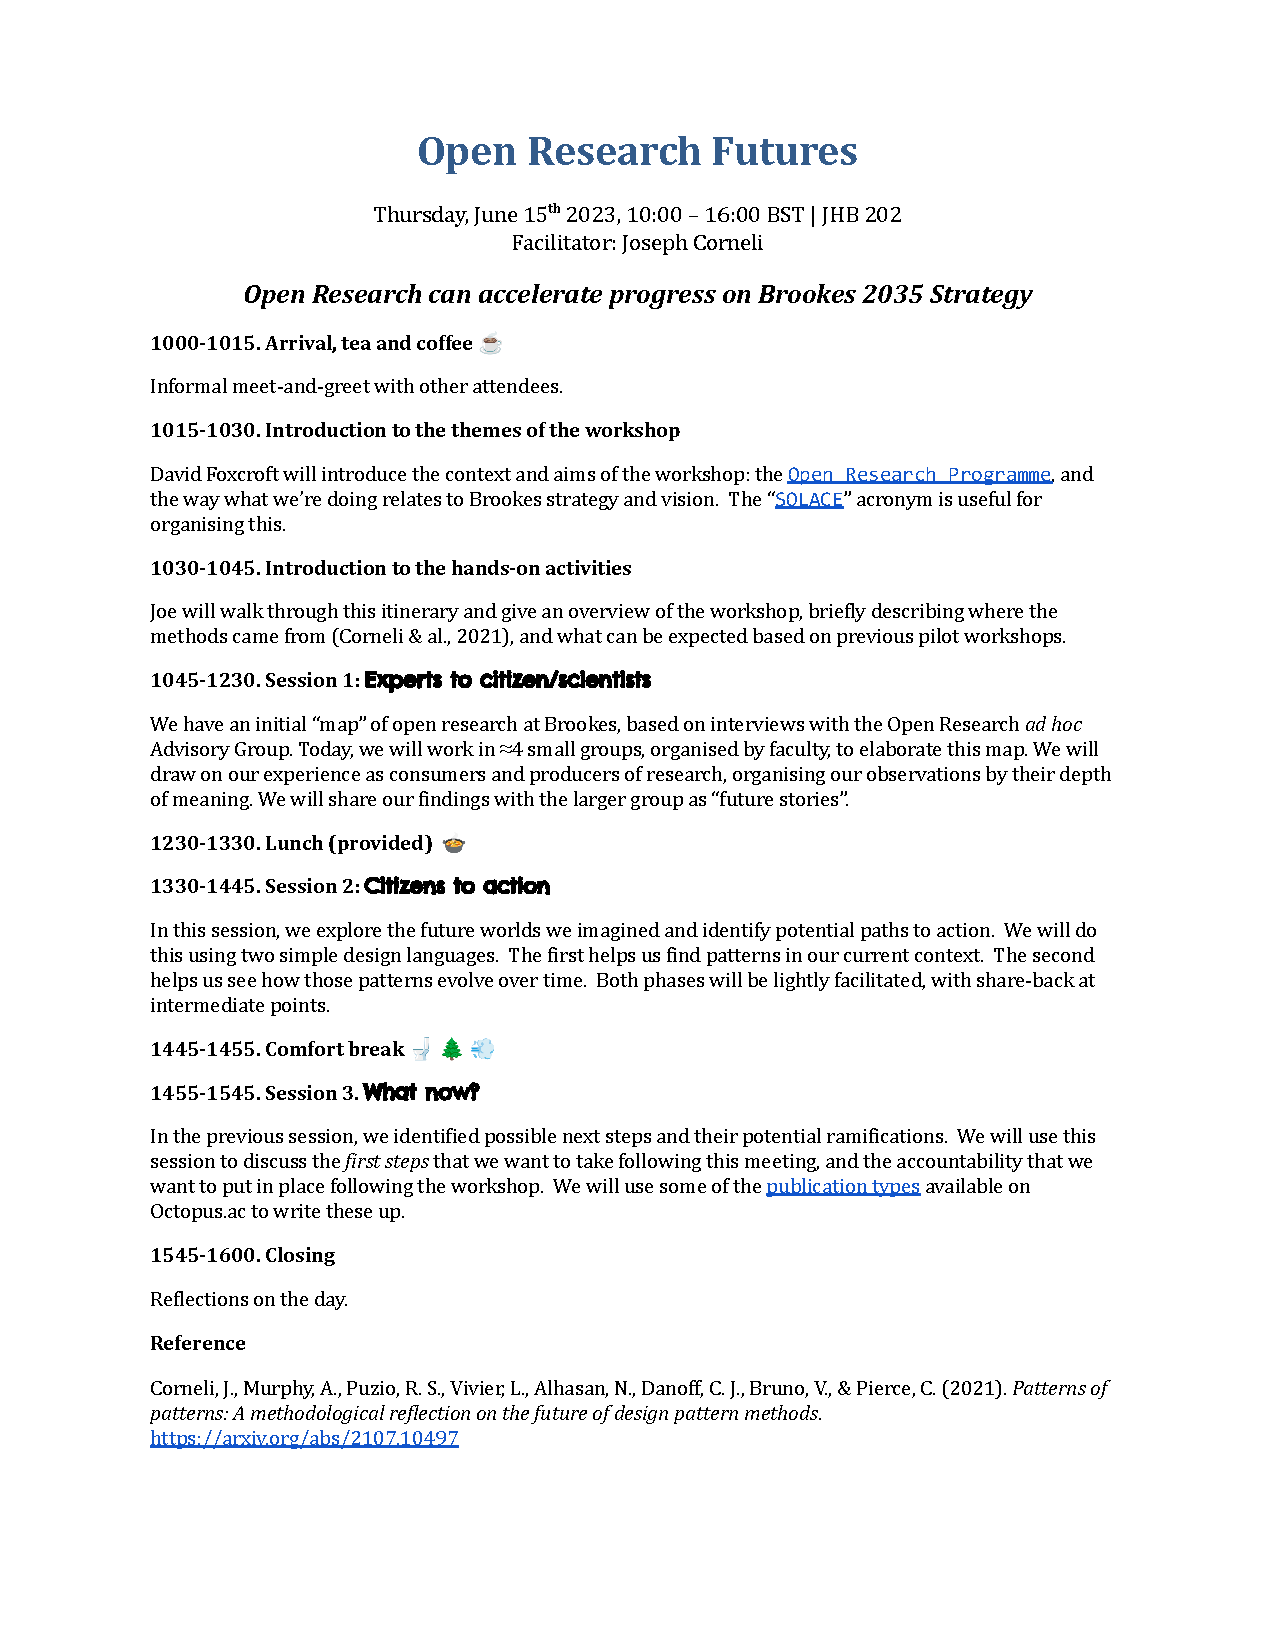
\includegraphics[width=\textwidth,trim={1cm 5.5cm 1cm 4.5cm},clip=true]{brookes}
\end{mdframed}

\clearpage

\subsection{Intermediate artifacts}

Figure \ref{brookes-workshop} shows how the {\sc Pattern Language
  Components} were used in the second phase of the workshop, building
on a CLA-based discussion that developed the {\sc Meaning Map} in the
workshop’s first phase (background, right).  In this case, the
keywords and manipulatives corresponding to {\sc Functional Roles}
(cf. Table \ref{mnemonic-for-manipulatives}) were not used to spell
out entire draft patterns (as in Figure
\ref{ExampleParticipantPattern}), but rather, to generate a network of
relations.

\begin{figure}[h]
\begin{tabular}{c@{\hspace{3em}}c}
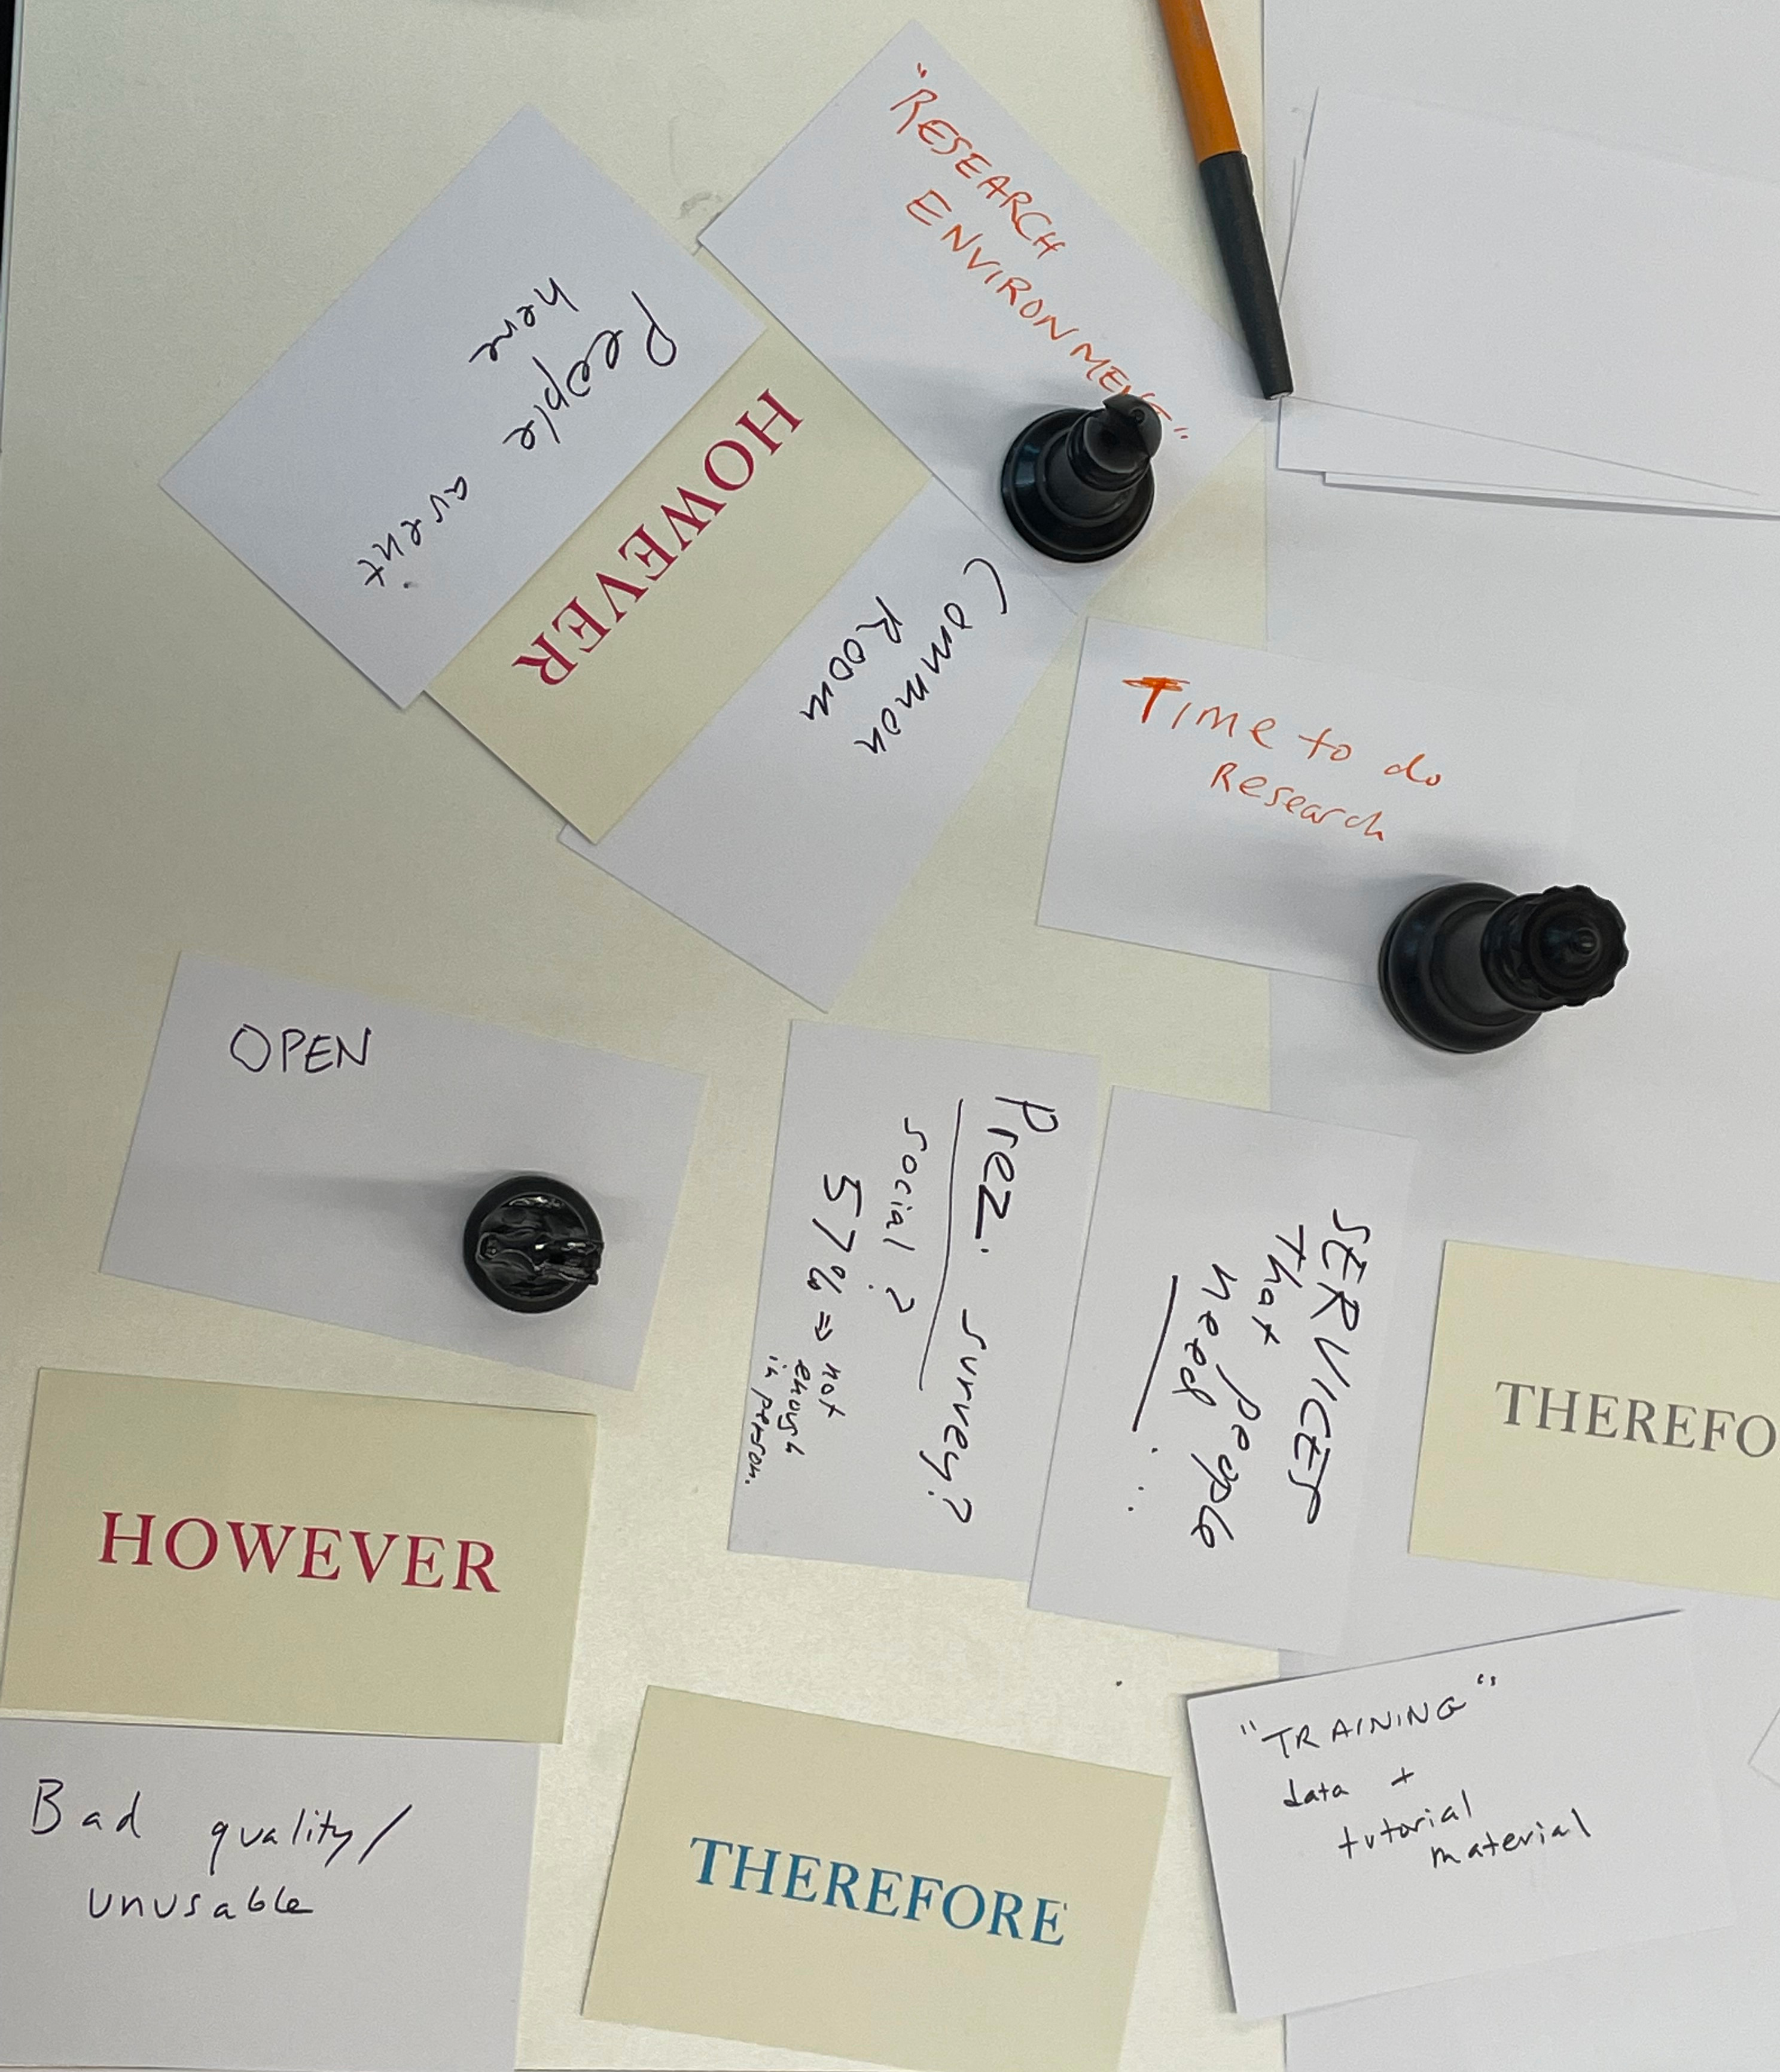
\includegraphics[trim={.2cm 0cm 0cm 2cm},clip=true,width=.4\textwidth]{fragment1.jpg}  &
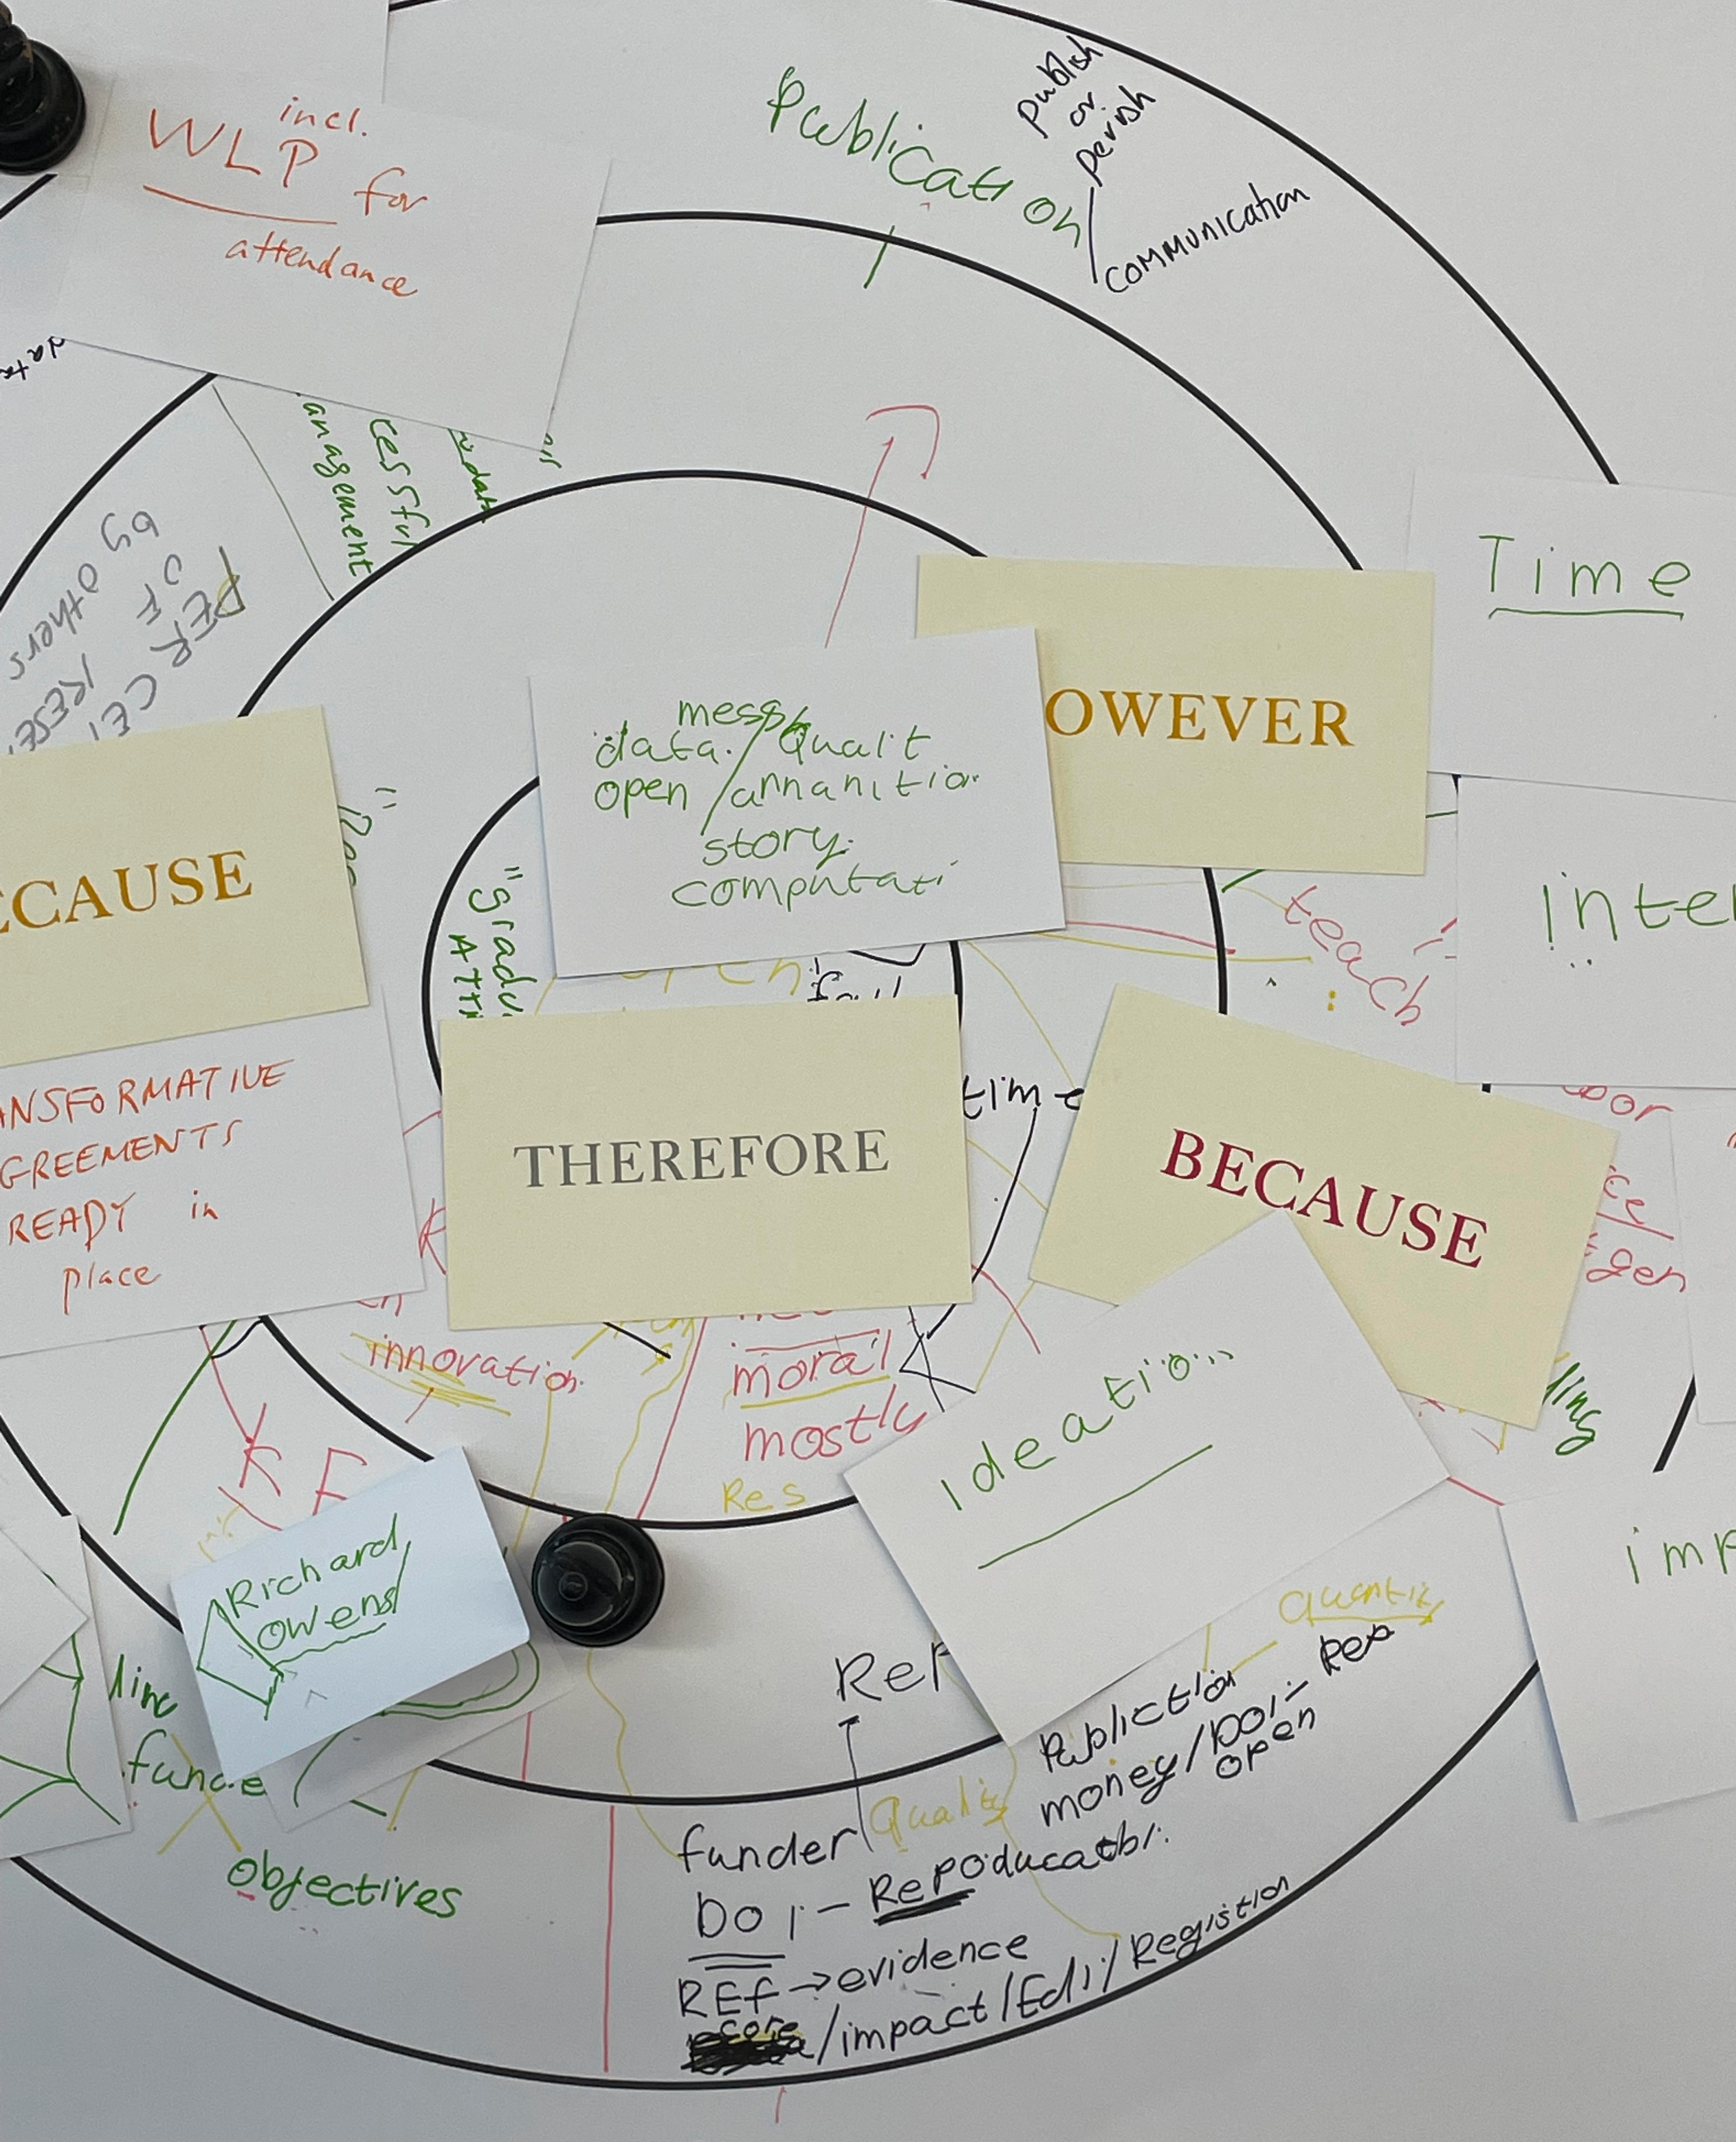
\includegraphics[trim={0cm 1.4cm 0cm 2cm},clip=true,width=.4\textwidth]{fragment2.jpg}
\end{tabular}
\caption{The {\sc Pattern Language Components} were used organically within the workshop.\label{brookes-workshop}}
\end{figure}

Figure \ref{Org-Roam-Screenshot} shows how material was then drawn
together, using Org Roam to analyze the workshop themes (per the {\sc
  Linker} pattern), further elaborating the {\sc Meaning Map}.
Contents of the paper-based diagrams, like those in Figure
\ref{brookes-workshop}, were condensed and edited in the digital
notes, rather than represented verbatim.  For example, the idea of
reintroducing a ``common room'' (Figure \ref{brookes-workshop}, left)
is folded into the ``Research Environment'' node, along with the
challenge of holding conversations when “people aren’t here” in
person.  The digital notes also provided an opportunity for
corrections, consolidation, and synthesis of links which hadn’t been
spelled out directly with the manipulatives. E.g., ``Richard Owens''
[sic] (Figure \ref{brookes-workshop}, right) is represented in the
digital notes as \emph{Richard Owen}, key proponent of responsible
innovation \cite{Owen2013}, within the ``responsible'' node.

The overall process illustrated in Figure \ref{Org-Roam-Screenshot}
moves in the opposite direction of \emph{Figures 3-7} of
\citet{iba2016pattern}, insofar as those figures complexify a tree as
a graph.  Here, we move from an interlinked graph of topics to a
summary map in tree form, represented here by the Outline of an Open
Research Action Plan node.  This process relates to the interplay of
informal and formal work, elaborated in Appendix
\ref{synthesis-of-form}.

In brief, the organic, playful, interactions within the workshop were
useful in creating the more formal output (a draft policy document)
precisely because these interactions were informed by a suitable
metalanguage, including the apparatus of Causal Layered Analysis, the
{\sc Pattern Language Components}, the {\sc Functional Roles}, the
{\sc Meaning Map}, and other patterns described so far in the paper.
By contrast, the acronym ``SOLACE'' mentioned in the itinerary—which
aims to describe an approach to research that is grounded in
organizational values “Success, Openness, Learning by doing,
Adaptability and Creativity, and Equal opportunity”
\cite{corneli-varuf}—was primarily useful for {\sc Context Setting}.
That level of analysis only provides a “mental picture”, in the terms
of \citet{alexander1964notes}.  A hypothetical Open Research Action
Plan based on stakeholder interviews and the “SOLACE” concept,
omitting the workshop experience, might express the university’s
values, but it would not draw on the same richness of meaning, nor the
same level of practical detail.

% If you imagine the nodes, they can be a litany, something we could go deeper into
% Imagine you rotate it 90°, you could visualise it in a different way: “pivot”
% This point that happened at any point in the process.
%—Any of these points becoming a ‘center’ of something else
% If I filter to only the nodes that are a distance 3 of this
% It has a 3D aspect; 

\begin{figure}[h]
  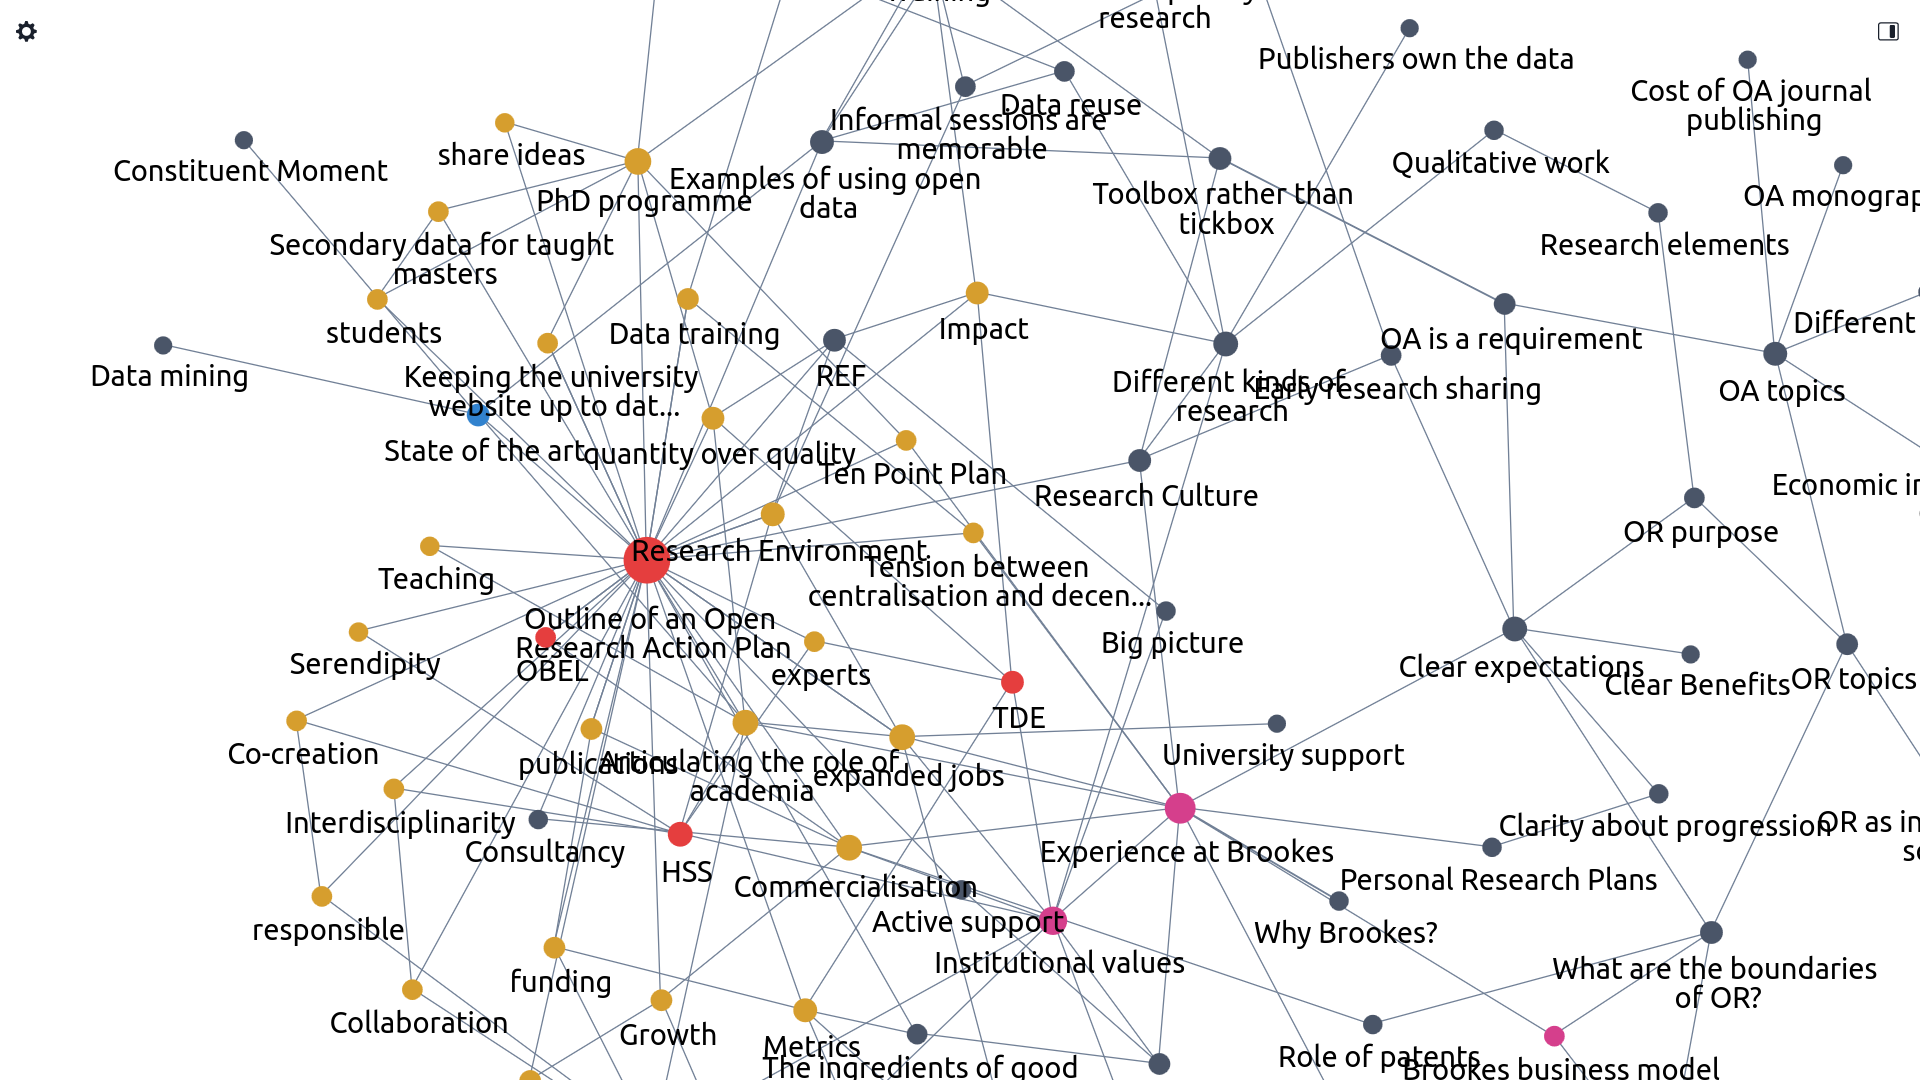
\includegraphics[width=\textwidth,trim={0 0 0 2cm},clip=true]{org-roam-screenshot.png}
  \caption{Screenshot of Org Roam UI, showing the development process
    leading to a draft Open Research Action Plan (ORAP).  Color-coding
    is: (Gray) Background themes and concepts based on interviews
    (cf. {\sc Do Your Research}); (Purple) Selected themes from that
    background material which became the focal themes in the workshop;
    (Yellow) Workshop themes and concepts; (Red) Key points of
    organization for workshop themes, including discussions per
    faculty as suggested by {\sc Structure Conversations}. The node
    “Outline of an Open Research Action Plan” includes the ORAP,
    instantiated here as a bullet-point outline, with links to all of
    the workshop outputs.
    \label{Org-Roam-Screenshot}}
\end{figure}

\subsection{Output Patterns}

\emph{The process of condensing wide ranging interviews and workshop
discussions into a draft report suggests the following broadly useful
pattern:}

\subsection*{💎 STRUCTURE OUTPUTS{\hfill\motor}}
Having gathered themes from a participatory project, they may have
some explicit (e.g., because of how the information was gathered,
cf. {\sc Structure Conversations}).  Additional structure can be
created, if you link intermediate artefacts into a relevant template.


\smallskip
\noindent\emph{Our way of working with {\sc Pattern Language
  Components} within this workshop suggests another pattern going in
the opposite direction of formality:}

\subsection*{💎 DESTRUCTURE PATTERNS{\hfill\cognitive}}
The {\sc Pattern Language Components} need not be used to articulate
entire patterns: a less formal discussion can surface useful meanings.


%% \subsection*{PLACARD: A Synthesis of PAR, CLA, and DPL}
%% \label{sec:orgd924cd6}
%% \label{methods_summary} We are now in a position to explain how PAR, CLA,
%% and DPL combine into one holistic pattern, in Leitner’s sense of a
%% complete methodic description \cite{leitner2015a}.  We will write this
%% down using the classic DPL format: describing the associated
%% \emph{context}, the \emph{problem} denoting a conflict, together with a \emph{solution}.
%% As it happens, the three acronyms introduced earlier can be combined and remixed
%% to provide a title for this pattern.
%% $$\textrm{PAR}+\textrm{CLA}+\textrm{DPL}=\textrm{PLACARD}$$
%% This accurately suggests that
%% the methods need not be run in a fixed order, but are interwoven together.
%% %\paragraph{PLACARD}
%% \label{sec:org958ff04}
%% \label{PLACARD}

%% \begin{itemize}
%% \item \textbf{Context}: In the course of working on a project: \emph{we use the PAR to get a sense of our working context}.
%% \item \textbf{Problem}: Although we may encounter many difficulties in this context, our effort to understand them faces a central \textbf{challenge}, namely the fact that the problems span different layers and scales of complexity, so it can be hard to understand where the difficulties actually come from: accordingly, \emph{we use the CLA to understand and frame the problems and their interconnections}.
%% \item \textbf{Solution}: Once we have grasped the problem, we need to elaborate an actionable solution that remains adaptable to ongoing changes in the context: \emph{we use DPL to elaborate the solution (returning to PAR and CLA as needed)}.
%% \end{itemize}


\section{Case Study 4: CIS 9590, Information Systems Development Project} \label{cis-case-study}

\subsection{Introduction to the course from the instructor, Mary Tedeschi}
% Mary please write in this file

CIS 9590 is Information Technology Project Design and Management is the  ``Computer Information Systems'' (CIS) capstone project course for the CIS major wherein the students will apply concepts and techniques from prior course work, to design, develop, and create an implementable application for a working information system of an actual business. It also focuses on the design and management of systems to meet the increased need for information within an enterprise. The course exposes students to the fundamentals of IT project management required for the successful implementation of IT-based systems. The course presents tools and technologies for project definition, work breakdown, estimating, planning and scheduling resources as well as monitoring and control of project execution. Students utilize knowledge gained from prior coursework, and work in groups to design and manage an Information Technology project.  During my first semester, Spring 2020, teaching with the students using whatever development tools they were familiar with, I noticed this to be a problem so with this knowledge I changed the course to require the use of Intel One API.  This did not get implemented until Fall 2021.  I actually taught the course three times before requiring students to use the same software tool uniformly.  The course was a 3 hour course, first face-to-face.  Then synchronous online only.  In Fall 2021 we changed to 75 minutes in person and online (hybrid).  Students had to self-teach Intel One API with the use of tutorials and a buddy system.  The students seemed to have the necessary skills to learn enough of the software to create an implementable application.  This semester, Spring 2023, the students really seemed to lack the coding skills.


\subsection{Our use of “Patterns of Patterns” within the course, by guest lecturers Raymond Puzio, Joe Corneli, and Charlie Danoff}
\label{pop1-in-cis9590}
We used the paper “Patterns of Patterns” as a focal text with three
successive cohorts of CIS 9590 students.  The course syllabus is
focused on developing group projects with a computer programming
component.  Our hope was that the topics in the paper would inspire
them with new ideas about design and collaboration.  We focus
primarily on the latest iteration of the course (Spring 2023), in
which we made the most explicit use of the methods described above.
Figure \ref{cis-9590-anticipations} shows some of our anticipations of
the relevant concerns that apply in this context.
Each semester, students asked many thoughtful \emph{questions} about the
paper; they also produced their own \emph{written response} to the
paper, engaging the original paper in depth; and in the latest run, we
offered some in-class \emph{exercises} based on the workshop methods
described above.  Reading these written responses showed that the
students had not only understood the main ideas of our paper, but
added to them.  In effect, they created alternative imaginaries for
the paper’s history and future.  For instance, in their 2022 ‘case
study’, they generated a “Recommendation and Implementation Plan”
which proposed specific actions which a group could take based on our
ideas; and, in 2023, the students produced a slide presentation based
upon our paper, exploring its relationship to themes such as “emerging
technology”.  It is worth highlighting that while our paper did touch
briefly on the theme of emerging technology, the students considerably
elevated the importance of that theme in their feedback.

\subsection{Experience report by CIS 9590 student, Kajol Khetan}\label{sec:kajol-report}

The PLACARD method emphasizes understanding the context, selecting an
appropriate language or languages for thinking about problems in that
context, and taking relevant actions to guide the development process.
In our project work, we adapted the CLA component of this framework by
identifying the layers relevant to our chosen problem, namely, to
create a website that allows users to discover nearby coffee shops
easily.  We identified the following layers for our analysis (each
with several facets, see Figure \ref{kajol-box}): User Interface,
Functionality, Data Flow, Infrastructure, and External Factors.

\begin{figure}[h!]
\begin{mdframed}
\textbf{User Interface Layer}

\textit{Analyzed user interactions}: Implemented an interactive map
interface using JavaScript and integrated the Google Maps API.

\textit{Designed elements}: Developed a responsive and visually appealing
layout with markers representing coffee shops on the map.

\textit{User experience}: Prioritized ease of use, ensuring smooth
navigation, intuitive filtering options, and clear visual cues.

\textbf{Functionality Layer}

\textit{Core features}: Enabled users to search for coffee shops based
on location and preferences.

\textit{Functions/modules}: Implemented search functionality, marker
clustering, and information display for each coffee shop.

\textit{User feedback}: Incorporated user feedback to enhance
features, such as real-time reviews and ratings integration.

\textbf{Data Flow Layer}:
Processed user inputs: Captured user location and
preferences to provide relevant search results.

\textit{Stored data}: Utilized a database to store coffee shop
information, such as names, addresses, ratings, and reviews.

\textit{Data display}: Dynamically populated the map and details
sections with data retrieved from the database.

\textbf{Infrastructure Layer}:

\textit{Technology stack}: Utilized HTML, CSS, JavaScript, and Google
Maps API for the front end; PHP and MySQL for the back end.

\textit{Compatibility}: Ensured cross-browser compatibility and
responsive design to cater to various devices.

\textit{Server setup}: Hosted the website on a reliable server with
efficient performance.

\textbf{External Factors Layer}:

\textit{User requirements}: Considered user preferences, such as
coffee shop categories (e.g., vegan-friendly, Wi-Fi availability).

\textit{Business goals}: Aligned with the goal of promoting local
coffee shops and providing a convenient user experience.

\textit{Market trends}: Incorporated emerging trends, such as
real-time user reviews and social media sharing.

\end{mdframed}
\caption{Layers in the analysis of a coffee discovery website\label{kajol-box}}
\end{figure}

CLA guides us to look for \emph{causal relationships} operating within
and between these layers.  In particular:
\begin{itemize}
  \item Changes in the User Interface layer influenced user engagement
    and ease of interaction.
  \item Adjustments in Functionality impacted the overall user
  experience and satisfaction.
  \item Data Flow optimizations directly affected the accuracy and
    relevance of coffee shop information.
  \item Infrastructure decisions impacted website performance and
    responsiveness.
  \item External factors influenced design choices and user
    satisfaction.
\end{itemize}

Our adaptation of Causal Layered Analysis led to a comprehensive
understanding of the website's components and their interdependencies,
and facilitated a structured approach to development.  The nearby
coffee shops website was successfully developed and deployed.  Users
can input their location and receive a map display of nearby coffee
shops, along with relevant information such as ratings, reviews, and
operating hours.  Our group’s process could be condensed into an
overall protopattern:

\subsection*{💎 ADAPT LAYERS AS NEEDED {\hfill \cognitive}}
%\textbf{Context}:
The project's context was to provide users with a simple, intuitive
platform for locating nearby coffee shops. Challenges inherent to this
problem included real-time data updates and dynamic user interactions.
We needed to select appropriate design and implementation
\emph{languages}, and plan and carry out suitable \emph{actions}.
%\newline \textbf{Languages}:
The project employed Python, SQL, and Google Maps API. Layer-based
analysis and design facilitates effective communication among team
members, enabling seamless collaboration.
%\newline \textbf{Actions}:
Design patterns such
as {\scitshape MVC (Model-View-Controller) architecture}, the
{\scitshape Observer} pattern for real-time updates, and the
{\scitshape Singleton} pattern for managing map instances were
integrated into the development process.


%% 6. Discussion:

%% The application of the CLA method facilitated a structured approach to
%% development, ensuring that project requirements were met while
%% adhering to best practices. The integration of design patterns
%% streamlined development, leading to a user-friendly and responsive
%% website.

%% 7. Lessons Learned:

%% Through the project, we learned the importance of selecting
%% appropriate design patterns based on the context and requirements. The
%% CLA method guided decision- making and enhanced project management,
%% resulting in a successful outcome. CLA highlighted the importance of
%% systematically analyzing and optimizing each layer for a cohesive and
%% effective user experience. Flexibility and adaptability were key in
%% addressing challenges and meeting user needs.


\subsection{Further proto-patterns describing the course experience, by CIS 9590 student, Manny Singh}\label{sec:manny-protopatterns}

%% Introduction:
%% During my final project class led by Professor Mary Tedeschi, the research paper 'Pattern of Patterns' and its authors played a pivotal role in shaping my project decisions. The authors' active engagement in our Zoom sessions provided invaluable insights into project layout, helped me avoid common mistakes, and encouraged a scalable and adaptable approach. Their active engagement and promises to come again in the following weeks to see progress on everyone’s individual project kept the butterflies, nervousness, and willingness to deliver all alive at the same time.

\emph{The following proto-patterns summarize one student’s reflection
on how our “active engagement and promises to come again in the
following weeks to see progress on everyone’s individual project kept
the butterflies, nervousness, and willingness to deliver all alive at
the same time.”  Further inline commentary expands and analyzes the
proto-patterns using {\sc Pattern Language Components}.}

\subsection*{💎 ENGAGEMENT AND GUIDANCE{\hfill \motor}}
The authors of ‘Pattern of Patterns‘ actively participated in our
class, to share expertise and create a collaborative learning
environment. Their presence allowed us to gain deeper insights into
the paper's concepts and methodologies, leading to innovative project
approaches. By closely studying the patterns of patterns identified in
their research, I gained a fresh perspective on project organization
and established a logical and coherent structure.


\smallskip
\noindent\emph{Notice that within this capsule summary there are at least two implied conflicts:}
\begin{itemize}
\item \emph{Team work is required HOWEVER the ways to scaffold effective collaboration are not entirely obvious;}
\item \emph{Project development is required HOWEVER project structure is not obvious.}
\end{itemize}
\emph{Our interactions with both the teacher and the students helped us theorize the confusion:}
\begin{itemize}
\item \emph{These difficulties exist BECAUSE participants do not have enough experience grappling with ‘worked examples’ (both learning best practices from successful examples, and learning by giving constructive feedback on less-successful examples).}
\end{itemize}
\emph{“Patterns of Patterns” provides some generic methods that can be applied to the domain-level problems.  Moreover, contact with the authors shifted the game, relative to simply reading the preprint.}
\begin{itemize}
\item \emph{THEREFORE, share some easy-to-understand general-purpose methods with novices, and put them in regular contact with people who have significant experience with problems in the domains of project management and collaboration.}
\end{itemize}
\emph{Thinking beyond the Spring 2023 CIS 9590 cohort to next steps, we need better ways to share this kind of experience:}
\begin{itemize}
\item \emph{SPECIFICALLY, can the Peeragogy project develop an internship/mentoring programme, and how would the design of such a programme be reflected in our design pattern catalogue?  (After the course, one of Mary’s students, Kajol Khetan, joined us as the first peeragogy intern.)  Respectively, can more touchpoints for mentoring and peer feedback be built into the CIS 9590 curriculum?}
\end{itemize}

\subsection*{💎 AVOIDING MISTAKES{\hfill \cognitive}}
The authors' insights helped me navigate common project development
pitfalls.  Through their emphasis on effective documentation, regular
testing, and thorough project planning, I was able to avoid costly
errors.  Their guidance ensured a consistent progress trajectory and
maintained the professionalism of my final project.


\smallskip
\noindent \emph{The nice features of “effective documentation, regular testing, and thorough project planning” might be interpreted in terms of PLACARD components:}
\begin{itemize}
  \item \emph{A project needs to be carried out HOWEVER it’s not clear what to do to make the project a success}
  \item \emph{BECAUSE projects have fairly well-known failure modes}
  \item \emph{THEREFORE teach and carry out ways to avert those
  failures: e.g., use Project Action Reviews to keep track of
  incremental steps in the development of the project; use Design
  Pattern Languages to design, build and evaluate prototypes; and use
  Causal Layered Analysis to integrate data from these to build an
  adaptable project plan that addresses a real problem.}
\end{itemize}
\emph{(That said, it would be helpful to offer more specific guidance, relevant to the novices’ working context.)}
\begin{itemize}
\item \emph{SPECIFICALLY, use a resource like
\citet{hoover2009apprenticeship} to flesh out this advice for future
CIS 9590 cohorts, and ask them to document the patterns they use.}
\end{itemize}

\subsection*{\normalsize{\emoji{gem}} SCALING AND ADAPTABILITY{\hfill \cognitive}}
‘Pattern of Patterns’ underscored the importance of scalability and
adaptability in project design.  By considering future technologies
and incorporating modular elements, I aim to seamlessly adopt new
advancements.  In particular, I focused on building a flexible
framework that could easily accommodate emerging technologies.


\smallskip
\noindent \emph{In the language we’ve been using internally,
“scalability and adaptability” sounds a lot like ‘working across
contexts’.}
\begin{itemize}
  \item \emph{We want a system that will adapt to situations we haven’t encountered yet HOWEVER we need something reasonably specific and concrete in order to work in any given context}
  \item \emph{BECAUSE we need to organize evolving complexity}
  \item \emph{THEREFORE develop a modular approach to design and development, and incorporate future scanning into the workflow}
  \item \emph{SPECIFICALLY let’s look for more ways to develop ‘alternative imaginaries’ for the Patterns of Patterns project}.
\end{itemize}

\subsection{Causal Layered Analysis of the CIS 9590 experience}

\begin{figure}[h]
  \begin{tabular}{cc}
    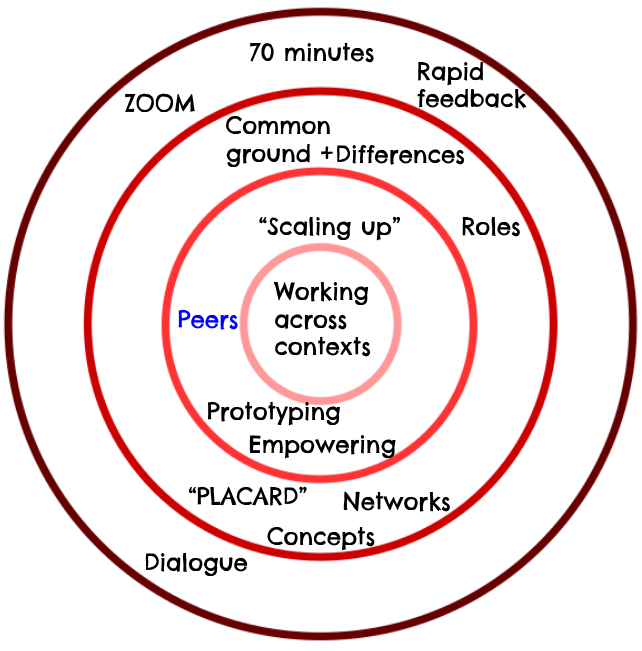
\includegraphics[width=.43\textwidth]{UsCLA.png} &
    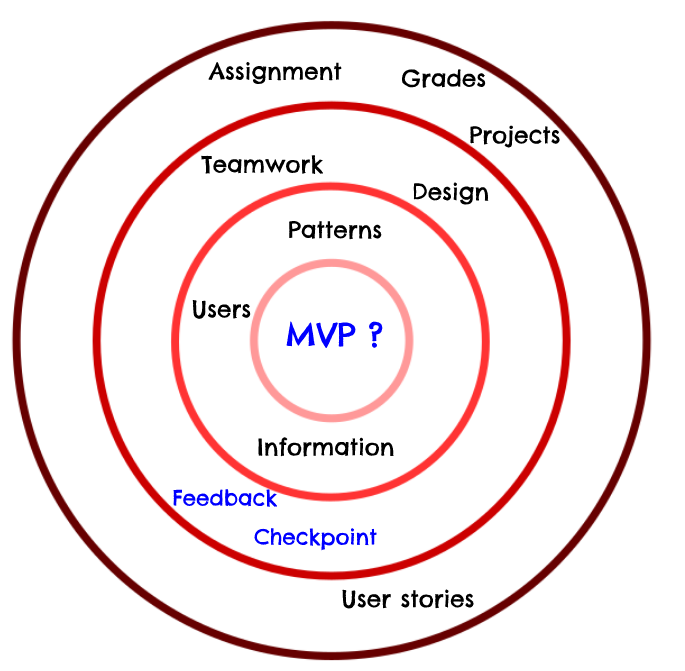
\includegraphics[width=.45\textwidth]{ThemCLA.png}
  \end{tabular}
\caption{Diagrams created before our first session with the CIS 9590 students, inspired by Causal Layered Analysis.  The diagrams describe our working context as guests in CIS 9590 (left), and our initial understanding of the students’ working context (right).\label{cis-9590-anticipations}}
\end{figure}

We conclude this section with a summary reflection on our use of
``Patterns of Patterns” within CIS 9590, using the (standard) Causal
Layered Analysis layers.  This is scaffolded by the two diagrams in
Figure \ref{cis-9590-anticipations}.

\subsubsection{Litany}
Initially our paper was introduced as a contemporary reading, relevant
to the Computer Information Systems (“CIS”) theme.  Mary chose a
contemporary paper in part because students would not be able to
“cheat” in their reports, because our paper wasn’t described
extensively on Sparknotes or similar.  Along with this (intentional)
challenge, CIS 9590 students encountered a range of more or less
predictable problems, e.g., many felt a lack of confidence with
coding.  The students came to the course with a variety of different
backgrounds (e.g., Python vs C++) which contributed to some friction
with this course.  As guest lecturers, our initial anticipations
(summarized in Figure \ref{cis-9590-anticipations}) didn’t precisely
match our reflections at the end of the course.  This suggests the
potential need for more design patterns.  With the benefit of
hindsight, next time we might elaborate on Manny Singh’s
proto-patterns to give them more specificity, and influence our
participation in future cohorts.  More broadly, we observe that when
\emph{working across contexts}, many of the ‘forces’ at work within a
given context are initially hidden to us.  For example, we didn’t
anticipate the students’ hesitance around coding, nor did we anticipate
their taking up the cause for emerging technologies around PLACARD
methods.

\subsubsection{System}
Whereas in our rounds of earlier participation we were more there for
enrichment, in the most recent semester, our contributions were more
closely integrated into the main activities of the course.  We
attended more sessions, including one in which we attempted to run a
short version of the workshop with attendees via Zoom.  Ongoing
interaction saw us in an ‘in residence’ role, advising on various
aspects of the projects.  Furthermore, Mary attended at least as many
meetings of the Peeragogy project (one of the centers of development
for PLACARD) as we attended sessions of the course, fostering an
exchange of ideas and viewpoints between these two contexts. In the
short term, this led to productive synergy and, in the long term,
could lead to our pedagogical and peeragogical initiatives becoming
more integrated into a larger system. This collaboration continued
post-semester, insofar as Mary invited the students to express
interest in possible internships in the Peeragogy project.

\subsubsection{Worldview}
Students were thinking about their future careers.  What they wanted
to get out of the course (e.g., becoming a well-paid data scientist or
business leader) at times had some friction with the practical reality
of the course requirements, in which they had to deliver a concrete
hands-on working project, without being able to rely on employees.
PLACARD wouldn’t be of much direct help with the technical challenges
they faced with the Intel One platform, but we hoped it would help
them organize their work in a sensible way.  The ideas underlying
PLACARD informed our contributions to the course at various levels;
for example, in a session with Mary in which we ‘workshopped’ CIS 9590
with other peeragogues, discussants suggested adding more touchpoints
for peer learning and feedback (\emph{\`a la} the PAR).  The two
diagrams in Figure \ref{cis-9590-anticipations} illustrates how
different meanings and priorities (including but not only at the
Worldview level) can lead to tensions or even outright conflict: this
suggests a paticularly salient role for DPLs in bridging between
domains.

\subsubsection{Myth}
A deep metaphor within the classroom setting is \emph{pedagogy}.
However, the methods that we brought to the course as guests were more
linked with our experience of \emph{peeragogy}.  In the new shared
context, these two perspectives begin to integrate.  Mary as a host
exercised the value of \emph{xenia} by bringing us into her course as
guests.  The possibility of student internships within the Peeragogy
project would create the reciprocal opportunity for further student
practice with CIS skills in an applied context, helping to build tools
and platforms for peer learning and peer production (including through
use of pattern methods).  Indeed, the particular combination of peer
learning and formal education developed here led us to wonder how far
off the Peeragogy project might be from being able to support informal
learning of relevant programming concepts (preliminaries to CIS 9590)
or applied computing projects (an analogue of CIS 9590).  The
students’ emphasis on the theme of ‘emerging technology’ suggested
that whatever synthesis develops, it may include significantly
upgraded technical components.  We’ve seen a corresponding need for
emerging methods, e.g., in Kajol Khetan’s suggestion to {\sc Adapt
  Layers As Needed}.




%% Conclusion:
%% The research paper 'Pattern of Patterns' and its authors significantly influenced my final project experience. Their engagement, guidance in project layout, avoidance of common mistakes, and focus on scalability and adaptability empowered me to make informed decisions. By observing patterns and applying their insights, I successfully developed a project that thrived in the dynamic landscape of technology. I am grateful for the authors' contributions, which shaped my final project journey under Professor Mary Tedeschi's guidance.

\section{Discussion}

We presented the patterns that we developed and used over successive
runs of our workshop, in approximately chronological order, duly
revised for publication and subsequent re-use.  Our accompanying
narrative showed how the application of certain patterns gives rise to
the ``seeds'' of new patterns.  It may now make sense to think of our
Open Future Design workshop methods as a nascent pattern language
which operationalizes the PLACARD pattern.  Our first workshop mixed
{\sc Pattern Language Components} with {\sc Functional Roles}, putting
participants in the thick of a pattern-related dialogue.  While this
led to interesting conversations, it was more work to extract any
patterns.  However, we did find some useful process patterns this way,
such as {\sc Increase Participant Control}.  We employed what we
learned in subsequent runs.  In the second workshop, a more distinct
use of the {\sc Pattern Language Components} helped the participants
come up with their own patterns.

There is an interesting interplay between the domain-level patterns
that were devised by workshop participants and the process-level
patterns that describe the workshop itself.  For instance, the
workshop setting is akin to a public space, and issues like {\sc
  Contested Space} would apply there, whenever different participants
have different conceptions of how they want things to go.  Further
development of the tools associated with the workshop might make it
even more of a public resource—somewhat like Wikipedia, but endorsing
the contribution of original research, rather than forbidding it.
This remark should simultaneously recall the analogy between wikis and
pattern languages \cite{cunningham2013a}, and frame the need for it to
develop.

In order for any pattern-informed research to work well, we should be
gathering evidence for or against the salience of the patterns that
are elaborated.  The Octopus\footnote{\url{https://www.octopus.ac/}}
platform mentioned in the itinerary for Case Study 3 uses several data
types that follow the rough outline of a scientific paper; amongst
them, the “Problem”, “Rationale”, “Method”, and “Results” components
are particularly familiar for pattern authors.  Much as Octopus
disaggregates research papers, our experience in Case Study 3 suggests
that when engaging with complex problems, it can be useful to {\sc
  Destructure Patterns} as well.

An archive of patterns and pattern components could be upgraded with
tools that go far beyond archival purposes.  Because of the particular
practical aims of the exercise, Figure \ref{Org-Roam-Screenshot} in
Case Study 3 centers on the “Outline of an Open Research Action Plan”
node, towards which the several layers of data-gathering and analysis
are all directed.  However, in principle, any one of the nodes could
itself become a center for further inquiry, e.g., in the first
instance, simply by restricting the graph to a neighborhood around
that node.  A shift in the analytic focus may also correspond to a
shift in the layers of analysis, for example what looks like
“litany-level” from one perspective may be viewed as a “system-level”
node from another.

\begin{figure}
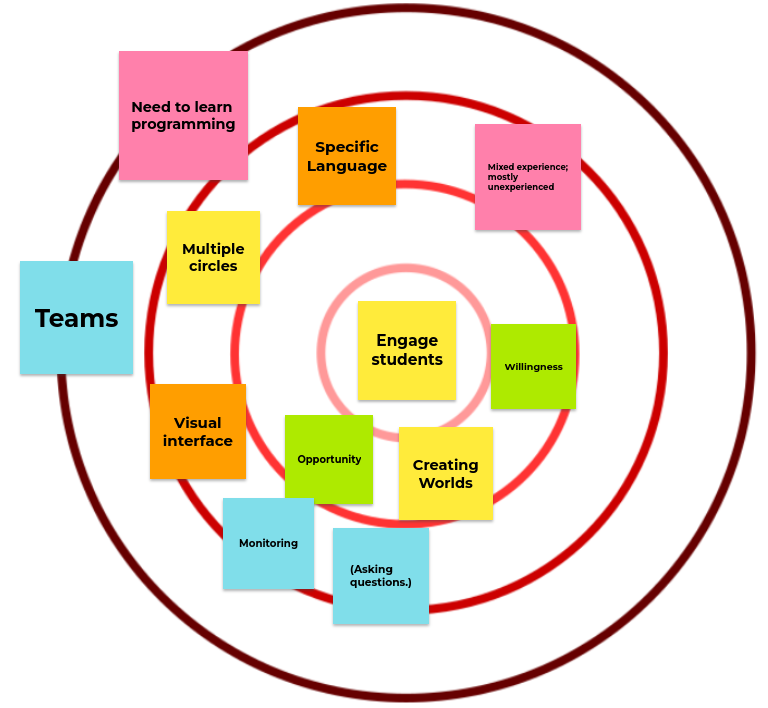
\includegraphics[width=.7\textwidth]{sridevi-course.png}
\caption{We used the CLA template to plan a future Introduction to Computing course for high school students\label{sridevi-course}}
\end{figure}

The foregoing remarks suggest a relationship between \emph{patterns}
and \emph{research} that should be pursued further.  As discussed in
Case Study 4 (and at length elsewhere in the literature) there is also
a fruitful relationship between \emph{patterns} and \emph{education}.
Our concluding case study illustates one way in which patterns can
bridge between education and research.  A further example is
warranted.  In Figure \ref{sridevi-course}, we show how our experience
with CIS 9590 could inform a future Introduction to Computing course
for high school students.  Here, part of the \emph{system} layer
envisions ‘multiple circles’ (i.e., multiple instantiations of the
four-layer CLA template) which would express the developing
perspectives in different groups of students collaborating together in
the course.  These would be integrated into one overall perspective
through a ‘monitoring’ interface used by the instructor, elaborating
on our aim of \emph{working across contexts}.



\FloatBarrier

%% (Another nice feature we can observe in this write-up is
%% that the {\sc Reflector} and {\sc Time Traveller} work as a pair,
%% since both are primarily sensory patterns, and similarly the {\sc
%% Analyst} and {\sc Linker} work as a pair of cognitive roles.)


\section{Summary}

The primary contributions made in this paper can be summarised as
follows:

\begin{itemize}
\item Table \ref{summary} pulls together the patterns we have
  described from across the separate case studies, and organizes them
  in groups, elaborating our previous use of “PAR”, “CLA”, and “DPL”
  methods (summarized in Section \ref{sec:org7c32ecc}) with \emph{a
  rounded outline of the purposes that sensory, cognitive, and motor
  methods serve when working with design patterns.}

\item Figure \ref{pattern-analysis} summarizes the patterns in a
  visual way, constituting a {\sc Meaning Map} for our “patterns of
  patterns”.  This visual summary in Figure \ref{pattern-analysis} is
  elaborated in textual form in Appendix \ref{cla-appendix}.  In
  short, like a round wheel that rolls better on round ball bearings,
  \emph{our analysis of the “Patterns of Patterns” can make work with
  patterns more efficient}.

\item Figure \ref{revised-cards} re-presents selected patterns from
  the paper in \emph{a practical format for use when co-designing
  future workshops, or other related interactions}.\footnote{``Open
  Future Design Workshop: Together with workshop participants, we will
  co-develop a Design Pattern Language for envisioning, exploring, and
  enacting the future.”  Wikimania 2023,
  \url{https://pretalx.com/wm2023/talk/WVLJRV/} (Recording:
  \url{https://www.youtube.com/watch?v=R2Sxs7lHv9w&t=13590s})} Whilst
  the collection of patterns has been refined through practice and
  critique, we make no claim of completeness.  “Blank” cards in Figure
  \ref{revised-cards} explicitly suggest that further patterns can and
  should be added.  \emph{Through our examination of {\sc Functional
    Roles}, we now have an improved understanding of how and when new
  patterns are likely to be needed, as well as how to develop them.}
\end{itemize}

\clearpage
\begin{table}[p]
\hspace{-1em}\begin{tabular}{rp{.82\textwidth}}
    PLACARD & ‘By using the PAR (or another sensory method), we are
    able to identify recurring themes.  Then, by using the CLA (or
    another cognitive method), we are able to organize these repeating
    themes in a structure that exposes the underlying trends, causes,
    and potential terminating states. With DPL (or another motor
    method) we can make what we have learned actionable.’ \cite{patterns-of-patterns-i}
\end{tabular}
  \begin{tabular}{rll}
Sensory: &&\\
&{\sc Dérive Comix}& ‘document what you see’ \\
&{\sc Share Back}& ‘individual groups should present key findings’\\
&{\sc Pilot to Anticipate}& ‘anticipate the issues likely to arise in future iterations’\\
&{\bfseries\scshape Time Traveler }& ‘provide historical context and
anticipate alternate futures’\\
&{\bfseries\scshape Reflector}& ‘appraise each developing scenario’\\
&{\sc Contested Space}& ‘each space need not to support every use equally’ \\
&{\sc Context Setting}& ‘describe the hoped-for outcomes’\\
&{\sc Do Your Research}& ‘start doing the research in a more centralized way’\\
%\hline
Cognitive: && \\
&{\sc Meaning Map }& ‘get everyone on the same page’\\
&{\sc Pattern Language Components }& ‘build patterns piece by piece’\\
&{\sc Facilitator Roles}& ‘structure the collection’\\
&{\bfseries\scshape Analyst }& ‘identify and orchestrate the dynamic network’ \\
& {\bfseries\scshape Linker}& ‘providing visualization of patterns and interconnections’ \\
&{\sc Funding of Public Space}& ‘create a register of impacts’\\
&{\sc Going Meta}& ‘explore how the project’s methods can be applied to
itself’\\
&{\sc Structure Conversations}& ‘structure the discussions around shared interests’\\
&{\sc Adapt Layers As Needed}& ‘layer-based analysis facilitates effective communication’\\
&{\sc Avoiding Mistakes}& ‘navigate common project development pitfalls’\\
&{\sc Scaling and Adaptability}& ‘aim to seamlessly adopt new advancements’\\
&{\sc Destructure Patterns}& ‘a less formal discussion can surface useful meanings’\\
%\hline
Motor: && \\
&{\sc Reinfuse Expertise }& ‘enable richer and more complex thinking’\\
&{\sc Functional Roles}& ‘introduce different perspectives’ (in bold here)\\
&{\bfseries\scshape Wrinkler}& ‘what might derail or counter the proposed solution’\\
&{\bfseries\scshape Stepper}& ‘decide which actions would be most useful’\\
&{\sc Increase Participant Control}& ‘participants should not remain only an audience’\\
&{\sc Rebalance Social Services}& ‘address complex local challenges’\\
&{\sc The Future Begins Now}& ‘take preliminary actions before leaving’\\
&{\sc Structure Outputs}& ‘link intermediate artifacts into a relevant template’\\
&{\sc Engagement and Guidance}& ‘create a collaborative learning environment’\\
  \end{tabular}
  \smallskip
  \caption{Thirty “Patterns of Patterns”\label{summary}}
\end{table}

\clearpage

\begin{figure}[p]
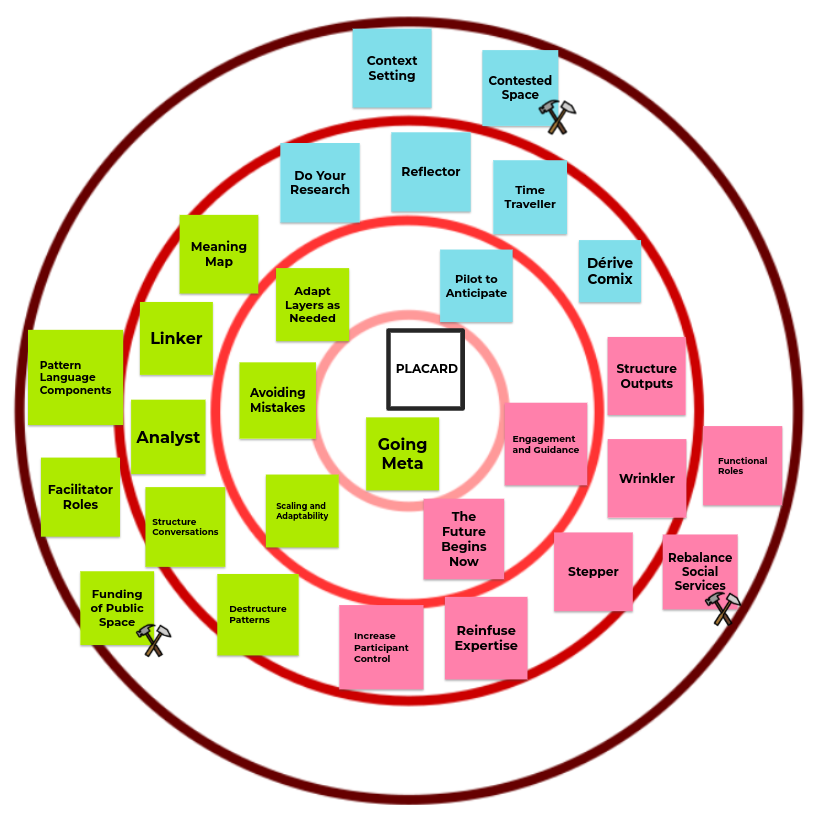
\includegraphics[trim={0 0 0 .1cm},clip=true, width=.9\textwidth]{revised-patterns-map.png}
\caption{Our “Patterns of Patterns” mapped to the four CLA layers. (Color code: blue=sensory, green=cognitive, red=motor.)\label{pattern-analysis}}
\end{figure}

\begin{figure}[h]
\begin{center}
\includegraphics[page=2,trim={1cm .5cm 1cm .5cm},clip=true, width=.85\textwidth]{./RPG-LaTeX-Template/cards.pdf}

\vspace{-.5cm}
  \noindent\includegraphics[page=3,trim={1cm .5cm 1cm .5cm},clip=true, width=.85\textwidth]{./RPG-LaTeX-Template/cards.pdf}
\end{center}
\vspace{-1cm}
\caption{Selected pattern cards, representing 14 patterns in manipulative form (with two “blanks”)\label{revised-cards}}
\end{figure}
\FloatBarrier

\section{Conclusion}

We carried out this work with the intention of designing the next
steps for our platform and process, and this seems to have been
successful.  As an immediate outcome, we developed the “PLACARD
workshop”—now retitled the “Open Future Design Workshop”—across
several successive runs, in different organizational contexts, in a
way that makes it fairly robust.  That success notwithstanding, the
scope of “Patterns of Patterns” was larger: our expressed aim was to
support collaboration across widely distributed contexts.

Although the work presented here was both wide-ranging and
participatory—and, indeed, we did prototype-level distributed-working
within teh workshops via the {\sc Share Back} pattern—we have not yet
implemented a fully distributed peer-to-peer collaboration platform
that can work effectively at a large scale.  However, considering the
paper as a whole, we have created something like a client-server
simulation of one.  For the facilitators, the workshop has repeated
with variation over time, allowing us to learn, gaining insights from
the workshop pilots which will contribute to the design of a platform
for distributed collaboration.

Alongside our concurrent prototyping efforts, one such crucial insight
is that the meta-level is just another domain.  All methodological
systems that aim to be practical—whether patterns of programs,
public health, open research, climate adaptation, or patterns of
patterns—should include predictions about the causal
connections between actions and measurements, and should incorporate
strategic intelligence to articulate action.

More work would be needed to fully describe our patterns’ application
domains, to build evidence of the kinds of results that can be
expected, and to fully describe their interconnections as a pattern
language.

Clearly, that be usefully complemented by supportive software
development.  For example, a not-so-distant future for Org Roam would
allow several facilitators to make notes in near real-time into a
shared map; and with further fine-tuning of the Emacs interface, a
similar workflow could be used directly by workshop attendees, even
across different contexts.  Many rich dialogues might ensue: already
we have seen the potential for fruitful cross-disciplinary interaction
between people from fields as disparate as future studies, health
sciences, open research, and information systems.  Existing systems
such as Alkemio\footnote{\url{https://alkem.io/}} are being built with
the need for collaboration across organizational boundaries in mind,
preferring \emph{challenge-focused} collaboration.

An approach centered on DPLs which work \emph{across related
challenges} would take that idea even further.  A knowledge management
tool like Org Roam could be augmented with additional “emerging
technologies” that make it more useful for the entailed complex
collaboration needs.  Domain-level design patterns outline potential
new behaviors; improved support for the process of gathering evidence
that those behaviors do (or do not) in fact work as intended is an
ambitious but logical ramification of the pattern method.  A further
step is needed to articulate the learning apparatus that underpins
such mechanisms in a computationally-coherent way.  The {\sc
  Functional Roles} we’ve set forth here provide an early informal
articulation of the process, and the connections to the Active
Inference Framework that we alluded to in Section \ref{role-of-roles}
could scaffold further, more formal, developments.
Although it is beyond the scope of the current paper, it would be
interesting build on these remarks in a way that integrates
programming- and software-specific design considerations, as
described, e.g., by \citet{felleisen2018design} and
\citet{lowy2019righting}.

Regarding our aim to support large-scale distributed collaboration,
whatever underlying formalism is used, and independent of which
technologies are used in the implementation, further work is needed to
identify analogies between action arenas, highlight the ramifications
of complex actions, show predicted costs and benefits, search for
tipping points that allow the effects of change to reach across level
boundaries, and surface new questions for consideration.  We have
begun (as we mean to carry on) by focusing on the development and
articulation of multi-purpose tools for thought that can help to
address these challenges.

\section*{Acknowledgements}
We thank the participants in our workshops, and the CIS 9590 students
who provided detailed feedback on “Patterns of Patterns” as it was
developing.  We wish to thank and acknowledge the funders who
supported our work.  The workshop described in Case Study 2 was
sponsored by a Springboard grant from the University of the West of
England; and the workshop described in Case Study 3 took place under
the auspices of the Research England REDF grant: “Growing and
embedding open research in institutional practice and culture”.  Kajol
Khetan’s contributions were supported by a Sidney and Laura Gilbert
Internship Award from Baruch College.  We would also like to thank our
PLoP 2023 shepherd Kiyoka Hayashi who gave detailed comments on
successive drafts of this write-up.  \textit{From Mary Tedeschi}: I
would like to thank Pai-Chun Ma, Nanda Kumar and Rudy Brown, who allow
me to be creative in my classroom.

\appendix
\renewcommand\thefigure{\thesection.\arabic{figure}}

\setcounter{figure}{0}
\section{Relationship to Alexander’s “Synthesis of Form”\label{synthesis-of-form}}
In this paper and the previous paper on “Patterns of Patterns” we have
considered the problems faced by groups of people organizing their
activities.  This can be usefully related to two diagrams from
Alexander's ``Notes on the Synthesis of Form'', recopied below as
Figure \ref{synthesis-diagrams}.  Parts a.-c. of this figure have two
columns corresponding to context/form (or in the terms Alexander uses
in his work on patterns: problem/solution), and one, two, or three
rows, corresponding to the ``actual world'', ``mental picture'' and
``formal picture''.  A design problem is posed at the level of the
actual world, say, ``build a house atop this hill'' or ``make a
celebration song''.

The design problem can be solved at one of the three levels.  The most
direct approach is to work in the actual world.  For instance, a
musician might pick up an instrument, start playing something, try out
different possibilities, modify notes or phrasings to make it sound
better, and so come up with a song.

At the level of ``mental picture'', a designer receives design
requirements which describe the problem, and produces a plan which
describes a solution.  For instance, the host of the party might make
a request ``Write a joyous song for alto voice accompanied by flute,
trumpet, and saxophone to celebrate the acceptance of our paper into
the conference.''  A composer might then sit down at a desk, away from
any instruments, and write out a score which would later be handed to
the singer and instrumentalists for performance.  Alexander points out
that there is a danger in this process: the composer would no longer
have the immediate feedback which comes from working directly in the
actual world.  Accordingly, the result might be a song that matches
the description, but doesn’t match the mood of the event.

Alexander’s proposed solution is to produce a formal picture of the
mental picture, and instead work with that formal picture.  For our
example, it might take the form of a suitably elaborate music theory,
one that includes concepts like ‘\emph{ballabile}’ (which indicates
that the song should be danceable).  More generally, we employ a
suitable metalanguage to reason about the mental representation; this
process of reasoning can then take the place of feedback from the
actual world in guiding and evaluating our designs.  For Alexander,
this consists of a set-theoretic formalization of design requirements
and potential misfits.

%% In the PLACARD setting, (CLA’s layers might correspond,
%% metaphorically, to the different voices used in the composition; a
%% analysis process akin to CLA might help to address goodness-of-fit.

Figure \ref{synthesis-diagrams}d refers to the process of design once
we have arrived at the ``formal picture'' level.  The left panel
represents the analytic process in which one decomposes a design
problem into subproblems and the right panel represents the
complementary synthetic process in which one successively combines
solutions to subproblems to arrive at a solution to the original
problem.  Alexander proposed a maximum entropy method for carrying out
the analysis and, in later works, introduced design patterns for use
in the synthesis; and ultimately, described 15 principles that could
guide a design at an even more abstract level.

The naive ``actual world'' approach (Figure \ref{synthesis-diagrams}a)
would be when a group takes a ``seat of the pants'' approach to
dealing with issues as they come up in the course of work.  PAR can
help to sketch a ``mental picture''.  CLA and DPL can be used as
techniques for analysis and synthesis at the ``formal picture'' level.
 Just as even a talented
musician without a solid grasp of music theory would be hard pressed
to compose an augmentation canon or symphony, so too we suggest that a
group which faces complex challenges may want to consider these
techniques for orchestrating their activities.  In sum, the methods
we’ve discussed can be used to operationalize a strategy that is at
the heart of Christopher Alexander’s oeuvre.

\begin{figure}[h]
\includegraphics[trim={3cm 7cm 3cm 3cm},clip=true, width=.9\textwidth]{appendix.pdf}
\caption{Diagrams from \emph{Synthesis of Form}\label{synthesis-diagrams}}
\end{figure}
\FloatBarrier

\section{SUPPLEMENT: Analysis: CLA applied to “Patterns of Patterns”} \label{cla-appendix}
\subsection{Litany: Understanding data, headlines, empirical world (short term change)}
Our Open Future Design workshop has evolved several features which are
retained across implementations.  Participants can expect {\sc
  Context Setting} from convenors/facilitators, as well as an
introduction to {\sc Pattern Language Components}, and {\sc Functional
  Roles}.  Workshop outputs are created collaboratively, with support
from people filling {\sc Facilitator Roles}.  We have seen that Open
Future Design process can help people articulate and grapple with
issues they see in their lives and communities, for example {\sc
  Funding of Public Space}, {\sc Contested Space} and the need to {\sc
  Rebalance Social Services}.  This list is representative rather than
exhaustive.  

\subsection{System: Systemic approaches and solutions (social system)}
The workshop proceeds through a combination of process steps ({\sc
  D\'erive Comix}, {\sc Meaning Map}, {\sc Reinfuse Expertise}),
supported by facilitators who work behind the scenes to {\sc Do Your
  Research}, and more overtly to {\sc Structure Conversations} and
{\sc Structure Outputs}.  Participants are aided by manipulatives
which help to {\sc Destructure Patterns}.  Facilitators will typically
fill the roles of {\sc Linker} and {\sc Reflector}, while participants
are invited to take on the roles of {\sc Analyst}, {\sc Time
  Traveler}, {\sc Wrinkler}, and {\sc Stepper}.  We aim throughout to
{\sc Increase Participant Control}, which can extend both to
participant co-design of the workshop experience itself (supported by
the patterns presented here), and to subsequent phases of work taking
place after the workshop that gather, process, and organize additional
data.

\subsection{Worldview: ways of knowing and alternative discourse}
Our methods express and communicate a worldview which works across
contexts to support {\sc Scaling and Adaptability}, offer {\sc
  Engagement and Guidance}, and help with {\sc Avoiding Mistakes}.
Our work is informed by Causal Layered Analysis and other structured
methods, however we encourage participants to {\sc Adapt Layers As
  Needed}.  One of the key purposes served by this paper is to
articulate a range of re-usable and re-mixable methods that can be
employed across sensory, cognitive, and motor domains.  The actions
considered within an Open Future Design workshop receive preliminary
testing and development inside the workshop itself: {\sc The Future
  Begins Now}. We encourage participants to {\sc Pilot to Anticipate}
beyond the workshop.  Taken together, our perspectives are linked with
the ethos of Peeragogy or “peer produced peer learning”.  Domain-level
issues may (usefully) mirror the workshop’s process-level patterns.

\subsection{Myths: metaphors and narratives (longer term change)}
We have flagged {\sc Going Meta} as the primary metaphor of this work,
in line with the series title, “Patterns of Patterns”.  The point is
not to be ‘meta’ just for the sake of it, but to find the
commonalities that reoccur across contexts, to build bridges between
different communities, and develop a reflective workflow that can be
improved as we go.  A suitable metaphor is found in the example of a
wheel that rolls more smoothly on round ball bearings.  This metaphor
helps to express the role that “Patterns of Patterns” play relative to
patterns themselves:
\begin{quote}
Technological progress is achieved through a dialectical relationship
between mediation (adaptation to the end terms: the path to be
travelled and the load to be carried) and autocorrelation, the
relation between the technical object and
itself. \cite{Simondon2005-pq}
\end{quote}
As a useful point of comparison, we observe that the “hierarchical
generative model capable of self-access” from
\citet{albarracin2023designing} is also borne from the addition of
reflective meta-layers, ascending from:

{
\renewcommand*{\arraystretch}{1.2}
\begin{tabular}{lllp{.37\textwidth}}
  &``\emph{What am I trying to do?}''&and&``\emph{What am I perceiving?}''\\
to:&``\emph{What am I paying attention to?}''&and&``\emph{What am I trying to pay attention to?}''\\
to:&``\emph{How aware am I of where my attention is?}''&and&``\emph{Am I trying to maintain awareness of my \phantom{X} attentional state?}''
\end{tabular}
}

\medskip
\noindent Although the language is different (cf.~{\sc Adapt Layers As
  Needed}), an analogy between these three layers and the litany,
system, and worldview layers of CLA could be noted.  Towards a
theorization of social intelligence, by applying PLACARD to itself (as
it were), {\sc Going Meta} allows us to \emph{reflect} on our
intention, \emph{understand} where we are in the process of
development we outlined, and \emph{articulate} a way forward.


\renewcommand\bibname{References}
\renewcommand\refname{References}

\bibliographystyle{ACM-Reference-Format-Journals}
\bibliography{./main.bib}



\begin{comment}
\section{Shepherd comments 1 Jul 2023, 05:43 and response}

\begin{leftbubbles}
\label{Q:developed-by-authors} Section4: Question regarding pattern contents: In section 3, it is mentioned that "We used design patterns directly when developing and running the workshops. A selection of these patterns are included here." Are the patterns presented in section 4 the same design patterns developed by the authors, or are they created by someone else?
\end{leftbubbles}
\begin{rightbubbles}
Most of the patterns in the Case Studies were developed by the
authors, a few were developed by workshop participants during the
workshop and only summarized here ({\sc
  \hyperref[pat:contested-space]{Contested Space}}, {\sc
  \hyperref[pat:funding-of-public-space]{Funding of Public Space}},
{\sc \hyperref[{pat:rebalance-social-services}]{Rebalance Social
    Services}}).  Regarding contributions from Manvinder Singh: he was
originally a ‘participant’, and then became an author.
\end{rightbubbles}

\begin{leftbubbles}
Additionally, the format of the "Selected Patterns for Case Study" in
section 4 varies (e.g., some have only summaries or start with
questions), which raises concerns. If these patterns were developed by
the authors, it should write patterns in a consistent format with
context, problem, and solution. Furthermore, it is necessary to
include the Forces that explain the causes of the problem and the
Consequences as potential results of implementing the solution.
\end{leftbubbles}

\begin{rightbubbles}
Personally, I (Joe) don’t fully agree with the suggestion to use
‘consistent format’ throughout the document.  The patterns are
presented at different levels of formality corresponding to their
stage of development.  Personally I don’t see forces, consequences,
and potential results as entirely necessary, though they might be nice
to have.  In particular, if the patterns aren’t understable in their
current format, they certainly need to be revised.  Let’s see if the
clarifications we’ve developed so far are enough.

What we’ve come up with, after consultation with the coauthors, is a
better explanation of what we aim to do with the patterns here (in the
Methodology section) and a lot more pictures that aim to illustrate
the points that are being made.  Hopefully this achieves most of the
additional clarity that was intended by the shepherd suggestion above.
%(One more quick point about forces: we talk briefly about how a force
%analysis is complicated by working across contexts in Section
%\ref{further-reflections}.)
\end{rightbubbles}

\begin{leftbubbles}
Regarding the structure: In the current paper, each subsection of
section 4 presents the Itinerary first, then presents the “Selected
Patterns for Case Study.” However, since the patterns are embedded
within the Itinerary without being presented beforehand, it becomes
unclear. It leads to confusion, such as in the case of
4.1.2. Considering the flow from the METHODOLOGY in section 3, it
might be more reader-friendly and coherent to present 4.1.1 as
"Selected Patterns for Case Study" and 4.1.2 as Itinerary. This way,
readers can follow along with the discovery of how the patterns shape
the itinerary. Additionally, assigning pattern numbers to each pattern
and including the number in parentheses after the pattern mentioned in
the itinerary would make it more comprehensible for readers. For
example, something like "Meaning Map (No.3) in the content of
Itinerary."
\end{leftbubbles}

\begin{rightbubbles}
I’ve restructured each subsection ‘in order’ with clearly delineated
inputs, process, and outputs.  {\large \emoji{check-mark}}
\end{rightbubbles}

\begin{leftbubbles}
4.1: Regarding DÉRIVE COMIX: The solution "Go for a walk or just look
out the window wherever you are, and document what you see” is
important for solving the problem. However, in the Itinerary, it is
mentioned to "Bring data: captioned mental images of “anticipation in
action” (feel free to refer to photos on your phone)," which does not
align with the solution of the pattern.
\end{leftbubbles}

\begin{rightbubbles}
Slightly reworded to make these align better. {\large \emoji{check-mark}}
\end{rightbubbles}

\begin{leftbubbles}
4.5: The subsection name of "Proto-patterns describing the experience,
by a CIS 9590 student, Manvinder Singh” seems to be unrelated to the
"CASE STUDIES” which is the name of section 4. It might be better to
present this as a separate section. Furthermore, the content written
here appears to be a summary of what was learned from the case studies
rather than patterns. If it is intended to be patterns, it is
necessary to include the context, problem, and solution.
\end{leftbubbles}

\begin{rightbubbles}
The \LaTeX\ section level was incorrect, which was the main source of
confusion here.  These are “outputs” from Case Study 4—not
reflections on all of the case studies.  That’s fixed now.  {\large \emoji{check-mark}}

(As for how formal we need to be about presenting them, see my comment
above for now.)
\end{rightbubbles}

\begin{leftbubbles}
Examples: AVOIDING MISTAKES, it is necessary to describe the effective
solutions and the potential problems that may arise if those solutions
are not implemented.
\end{leftbubbles}

\begin{rightbubbles}
I’ve presented the material in both proto-pattern form and expanded
using pattern language components; I think that’s the right level of
detail for now. {\large \emoji{check-mark}}
\end{rightbubbles}

\section{Shepherd comments 3 Aug 2023, 15:58 and response}

\begin{leftbubbles}
The BACKGROUND and METHODOLOGY are written more detailed than before, which makes it easier to understand what you created and how it is created.
\end{leftbubbles}

\begin{rightbubbles}
{\large \emoji{thumbs-up}}
\end{rightbubbles}

\begin{leftbubbles}
section3: The explanation of the diamond mark is written as a difference of the writing style of the patterns, but as I read the paper, I wondered if the patterns with diamonds are also new patterns. If the pattern shown with the diamonds mark was created by the workshop, that should be included as a supplemental explanation.
\end{leftbubbles}

\begin{rightbubbles}
I introduced the separate {\normalsize \emoji{pick}} marker to distinguish those
patterns which were created by workshop participants.  Since we are
not presenting the exactly as they appeared in the workshop, they
could be presented in either pattern or proto-pattern form.  For now,
I’ve chosen to present them as proto-patterns, so the three patterns
that are concerned \emph{also have the} {\normalsize \emoji{gem}} \emph{marker} (see page \pageref{mnemonic-for-stepper}). {\large \emoji{check-mark}}
\end{rightbubbles}

\begin{leftbubbles}
Section4:DÉRIVE COMIX: It says "If you have a group BUT everyone has their own experiences" as the problem, but why is everyone has their own experiences a problem?  Is it a problem that each person has different experiences, so their thoughts about the future are diverse, and it is difficult for the group to agree on a single scenario for the future?, or is it a problem that it is difficult to understand each other's future scenarios?
\end{leftbubbles}

\begin{rightbubbles}
The diversity of perspectives in the group is really a good thing, since it can contribute to a richer meaning map!  As such this is an opportunity.  In the revised description of {\sc Pattern Language Components} for some wordsmithing related to how the “problem” language of DPL can be confusing for participants!  In {\sc D\'erive Comix}, the problem is really that “the group has been identified BUT the members don’t know each other well yet, and accordingly each has their own separate experience, and the group has no concrete shared meanings”... so I’ve included that revised text! {\large \emoji{check-mark}}
\end{rightbubbles}


\begin{leftbubbles}
MEANING MAP (c): What is the problem with "everyone has their own experience"?
\end{leftbubbles}

\begin{rightbubbles}
Again, this is mostly an opportunity: and the wording needs to be
clarified, and I’ve tried to do so! {\large \emoji{check-mark}}
\end{rightbubbles}

\begin{leftbubbles}
REINFUSE EXPERTISE: What is the problem with “If everyone has experience as a citizen BUT they also have expertise”?  Is it a problem that because we have a specialized area of expertise, they can only come up with opinions that are limited by that expertise, and the variety of ideas becomes narrower?
\end{leftbubbles}

\begin{rightbubbles}
That’s certainly one part of the problem.  If people just share
information with other experts, the discussion can become “siloed”.
The problem is how to overcome this tendency.  The idea in {\sc
  Reinfuse Expertise} is to overcome it by bringing together with
people who have different expertise, getting them onto the same page
as citizens, and only \emph{then} turning to their expertise.  I’ve
tried to revise the pattern to clarify this. {\large \emoji{check-mark}}
\end{rightbubbles}

\begin{leftbubbles}
PATTERN LANGUAGE COMPONENTS: What is the meaning of “Dynamic
keywords”? I cannot get that However or BECAUSE is written as Dynamic
keywords.
\end{leftbubbles}

\begin{rightbubbles}
What’s important is that the keywords are \emph{neutral}, rather than
dynamic.  Indeed, I’ve forgotten what ‘dynamic’ was supposed to mean!
So, I’ve tried to clarify what’s going on in the pattern text.
Basically, if we start with a ‘problem’ (as in standard DPL language),
then people often object that they don’t want to focus on problems,
but rather on challenges, or even better, on solutions!  However, DPL
does have ‘conflicting forces’ at the core: so we need to a way for
people to talk about conflict, without getting frustrated.  That’s
what this pattern is trying to do. {\large \emoji{check-mark}}
\end{rightbubbles}

\begin{leftbubbles}
Figure 1 makes it easy to understand the pattern at a glance and it is
good that you included pictures related to the patterns in the figure
1. However, I feel that there is a disconnect between the pictures and
the content of the pattern. It would be better to make the pictures
more consistent with the content of the pattern. And the “Projection
Action Review” came out suddenly, and I wondered where it came from. I
also wonder why this pattern is only in different color, and why
PATTERN LANGUAGE COMPONENTS and FUNCTIONAL ROLES aren’t included in
the Figure 1.
\end{leftbubbles}

\begin{rightbubbles}
The aim of Figure 1 is primarily documentary, so I would only want to
narrate it differently—rather than change the contents.  I’ve added
some clarifying comments about that figure (e.g., explaining why a
different color was used, and also explaining that some of the
patterns used here are after-the-fact descriptions of what we did on
the day).  I provided a link to the full set of cards shared with
participants in a footnote. {\large \emoji{check-mark}}
\end{rightbubbles}

\begin{leftbubbles}
I really like the diagram in Figure 2 that shows the relationships
between sensory, cognitive, and motor patterns. It would be better to
describe this in the sentence and refer to Figure 2.
\end{leftbubbles}

\begin{rightbubbles}
We modified the picture slightly so that it is a bit simpler, and made
the accompanying text more to the point. {\large \emoji{check-mark}}
\end{rightbubbles}

\begin{leftbubbles}
section5: I didn't catch who Abby Tabor was for a moment, so it would be more helpful to the reader to include a word like "the auther" or "professor", which would identify someone.
\end{leftbubbles}

\begin{rightbubbles}
Added ``coauthor” to explain her role in the paper. {\large \emoji{check-mark}}
\end{rightbubbles}

\begin{leftbubbles}
I could not see why the patterns are presented based on the chess set
so it would be helpful to have a more detailed explanation about the
reationships between pattern and chess set.
\end{leftbubbles}

\begin{rightbubbles}
I added a new Table \ref{mnemonic-for-manipulatives} which explains
the relationship to the chess pieces.  Although it wasn’t specifically
requested in your shepherding remarks, I’d also like to point to Table
\ref{active-inference-factors}, which re-describes the main roles in
more theoretically-salient terms. {\large \emoji{check-mark}}
\end{rightbubbles}

\begin{leftbubbles}
Figure 3 came out suddenly, but which sentence is it referred to in? It is good to have many figures in the paper, but it is better to explain what they are about in the sentences. Figures are to supplement the sentences written in the body of the paper, so if there are no sentences that refer to the figure, the figure will not be valid.
\end{leftbubbles}

\begin{rightbubbles}
  I’ve checked in Emacs, using \texttt{occur}, that the figures and
  tables are all referenced in nearby text.  The text should now be
  readable in a stand-alone fashion (i.e., without the
  figures). {\large \emoji{check-mark}}
\end{rightbubbles}

\end{comment}
\end{document}
